\documentclass[usenatbib]{mn2e} 
\usepackage{amsmath} 
\usepackage{amssymb} 
\usepackage{graphics}
\usepackage{graphicx}
\usepackage{epsfig}  
\def\be{\begin{equation}}
\def\ee{\end{equation}}
\def\ba{\begin{eqnarray}}
\def\ea{\end{eqnarray}}

\newcommand{\documentname}{paper~}
\newcommand{\match}{{\tt match}~}
\newcommand{\apj}{ApJ}  
\newcommand{\apjs}{ApJS}  
\newcommand{\apjl}{ApJL}  
\newcommand{\aj}{AJ}  
\newcommand{\mnras}{MNRAS}  
\newcommand{\mnrassub}{MNRAS accepted}  
\newcommand{\aap}{A\&A}  
\newcommand{\aaps}{A\&AS}  
\newcommand{\araa}{ARA\&A}  
\newcommand{\nat}{Nature}  
\newcommand{\physrep}{PhR}
\newcommand{\pasp}{PASP}    
\newcommand{\pasj}{PASJ}    

\newcommand{\kms}{\,km~s$^{-1}$}
\def\squig{\sim\!\!}
\newcommand{\LCDM}{$\Lambda$CDM~}
\newcommand{\beq}{\begin{eqnarray}}  
\newcommand{\eeq}{\end{eqnarray}}  
\newcommand{\zz}{$z\sim 3$} 
\newcommand{\avg}[1]{\langle{#1}\rangle}  
\newcommand{\ly}{{\ifmmode{{\rm Ly}\alpha}\else{Ly$\alpha$}\fi}}
\newcommand{\hMpc}{{\ifmmode{h^{-1}{\rm Mpc}}\else{$h^{-1}$Mpc }\fi}}  
\newcommand{\hGpc}{{\ifmmode{h^{-1}{\rm Gpc}}\else{$h^{-1}$Gpc }\fi}}  
\newcommand{\hmpc}{{\ifmmode{h^{-1}{\rm Mpc}}\else{$h^{-1}$Mpc }\fi}}  
\newcommand{\hkpc}{{\ifmmode{h^{-1}{\rm kpc}}\else{$h^{-1}$kpc }\fi}}  
\newcommand{\hMsun}{{\ifmmode{h^{-1}{\rm {M_{\odot}}}}\else{$h^{-1}{\rm{M_{\odot}}}$}\fi}}  
\newcommand{\hmsun}{{\ifmmode{h^{-1}{\rm {M_{\odot}}}}\else{$h^{-1}{\rm{M_{\odot}}}$}\fi}}  
\newcommand{\Msun}{{\ifmmode{{\rm {M_{\odot}}}}\else{${\rm{M_{\odot}}}$}\fi}}  
\newcommand{\msun}{{\ifmmode{{\rm {M_{\odot}}}}\else{${\rm{M_{\odot}}}$}\fi}}  
\newcommand{\lya}{{Lyman$\alpha$~}}
\newcommand{\clara}{{\texttt{CLARA}}~}
\newcommand{\rand}{{\ifmmode{{\mathcal{R}}}\else{${\mathcal{R}}$ }\fi}}  
\newcommand{\Lsun}{\mbox{\,$L_{\odot}$}}
\newcommand{\like}{\mathscr{L}}
\newcommand{\bftheta}{\mathbf{\Theta}}
\newcommand{\degree}{\ensuremath{^\circ}}
\def\spose#1{\hbox to 0pt{#1\hss}}
\def\simlt{\mathrel{\spose{\lower 3pt\hbox{$\mathchar"218$}}
     \raise 2.0pt\hbox{$\mathchar"13C$}}}
\def\simgt{\mathrel{\spose{\lower 3pt\hbox{$\mathchar"218$}}
     \raise 2.0pt\hbox{$\mathchar"13E$}}}
\font\smcap=cmcsc10

\begin{document}

\title[Dark Matter Halo Mass for LAEs  at $z=3.1$]{Using cosmic
  variance to constrain the dark matter halo mass of Lyman-alpha
  emitting galaxies at $z$=3.1} 
  
\author[~J.~E. Forero-Romero and J. Mejia]{
\parbox[t]{\textwidth}{\raggedright 
Jaime E. Forero-Romero$^{1}$ and
Julian Mej\'ia$^{2}$ 
}
\vspace*{6pt}\\
$^{1}$ Departamento de F\'{i}sica, Universidad de los Andes, Cra. 1
No. 18A-10, Edificio Ip, Bogot\'a, Colombia \\
$^{2}$ --}

\maketitle

\begin{abstract}
We use cosmological N-body simulations to find the characteristic mass
of dark matter halos hosting Lyman-Alpha Emitting (LAE) galaxies at a
redshift of $z=3.1$. The method is based on matching the statistics
for the number density between mock and observed fields. The mock
catalogs are constructed using a simple model where a dark matter halo
can only host one LAE with a probability $f_{\rm occ}$ if its mass is
found withing a certain range mass range delimited by two threshold
values, $M_{\rm min}$ and $M_{\rm max}$. We find that the most of the models that
are consistent the observed cosmic variance statistics are those with
halo masses in the range $10.5 < \log_{10} M_{\rm  min}/hMsun < 11.5$
and $\log_{10} M_{\rm max}/\hMsun < 13.5$ with and occupation fraction
that scales as $f_{\rm occ}=$. We explore three additional constraints
to narrow down these range: the number of mocks consistent with 
observations, observational constraints on the occupation fraction and
the angular correlation function. The first two conditions narrow down
the space parameter to $M_{\rm min}=$ and $M_{\rm max}$, $f_{\rm occ}$. The angular
correlation function does not add a significant constraint due to the
cosmic variance in the small angular fields where this statistics has
been computed so far. We make available the mock data for the best
models in a public repository. Implications for galaxy formation
models? 
\end{abstract}

\begin{keywords}
{galaxies: kinematics and dynamics, Local Group, methods:numerical}
\end{keywords}


\section{Introduction}

Lyman-$\alpha$ emitting galaxies (LAEs) have become in the last decade a 
central topic in studies of structure formation in the Universe. They 
are helpful in a diverse range of fields. LAEs can
be used as probes of reionization \citep{Dijkstra11}, tracers of
large scale structure \citep{Koehler2007}, 
signposts for low metallicity stellar populations and markers of the
the galaxy formation process through cosmic history \citep{ForeroRomero2012}.  


At the same time, theoretical and observational developments have
contributed to the emergence of a paradigm to describe structure
formation in a cosmological context. In this context it is considered
that dominant matter content of the Universe is to be found in dark
matter, whereby each galaxy is hosted by larger dark matter structure
known as a halo. 

Most models of galaxy formation find that the mass of the halo can be
used to predict properties of the galaxy such as its stellar mass and
star formation rate \citep{Behroozi2012}. Processes that regulate the
star formation cycle are also though to be strongly dependent on its
mass. Furthermore, the spatial clustering of galaxies on large scales
is entirely dictated by the halo distribution.  For the reasons
mentioned above, finding the typical dark matter halo mass hosting
LAEs represents a significant step forward to understand the nature of
this population in the context of Lambda Cold Dark Matter
($\Lambda$CDM) paradigm.  

Some theoretical approaches to this problem have been based on a
forward modeling. Starting from the DM halo population, the
corresponding intrinsic star formation properties are infered and
statistics such as the luminosity function, the correlation function
and the equivalent width distributions. Such modelling has been
implemented from analytic considerations, semi-analytic models
 and 
full N-body hidrodynamical simulations
\citep{Dayal2009, ForeroRomero2011, Yajima2012, ForeroRomero2012} . 

Added to the uncertainties in the astrophysical processeses describing
star formation in galactic populations, a highly debated steps in this
approach is the calculation of the fraction of Lyman-$\alpha$ photons
that escape the galaxy to the observer. Given the resonance nature of
the line, the radiative transfer of Lyman-$\alpha$ is sensitive to the
density, temperature, topology and kinematics of the neutral Hydrogen
in the interstellar medium (ISM) \citep{Neufeld1991, ForeroRomero2011,
Laursen2013}.  

This complexity makes the use of monte-carlo simulations for the
radiative transfer a required tool to obtain physically sound results,
although the degeneracy in the physical parameters involved in the
problem makes it difficult to achieve a robust consensus on what is
the theoretical expected value for the Lyman-$alpha$ escape fraction
in high redshift. 


Throughout this \documentname we assume a $\Lambda$CDM cosmology with the
following values for the cosmological parameters, $\Omega_{m}=0.27$,
$\Omega_{\Lambda}=0.73$ and $h=0.70$, corresponding to the matter
density, vacuum density and the Hubble constant in units of 100 km
s$^{-1}$ Mpc$^{-1}$. 

\section{Methodology}
In this \documentname we constrain the typical mass of dark matter halos
hosting LAES at $z=3.1$. Our model is based on the number density
information obtained in the recent large scale survey presented by XXX
where XXX LAEs are detected over 7 fields of $\sim 46 \times
35$Mpc$^{2}h^{-2}$ in area comoving in area corresponding to observed
fields of $XXX$ deg$^{2}$.  

Both the spatial distribution and luminosities of the galaxies have,
at least in a statistical sense, informatio to constrain theoretical
model of LAEs. The most detailed theoretical models are also faced to
diverse physical and astrophysical uncertainties in obtaining
statistical prediction for the Lyman-alpha line. This uncertainties
are largest impediment to consruct an ab-iitio model for LAEs.  

In this \documentname we want to step back and reduce the complexity of our
model, with the sole objective of reproducing the cosmic variance in
the number density of LAEs. Afterwards we will interpret the
implications of this result for physical models for Lyman-alpha
emitting galaxies. 

Our model is based on the predictions of a large volume high
resolution N-body simulation describing the gravitational dynamics of
dark matter. We do not have an strong bias towards the theoretical
expectation of what the mass of the dark matter halo hosting the
galaxy should be.  Instead, we fully explore the parameter space of
our simplified model. The only cut we impose is that observed LAEs do
not reside in dark matter halos with masses less than 10$^{10}$
\hMsun [citation].  


In the following subsections we describe the most relevant features of
the observational data, the N-body simulation we use, our model and
its parameters together with the method to compare its predictions
against observations. 

\subsection{The Observational Constraints}

Our observational reference are the recently published results of a
panoramic survey of LAES at $z=3.1$ by \cite{Yamada2012}. This survey
was conducted with the Subaru 8.2m telescope and the Subaru Prime
Focus Camera, which has a field of view covering $34\times 27$ arcmin,
corresponding to a comoving scale of $46\times35$ Mpc $h^{-1}$ at
$z=3.09$. The narrow band filter is centered at $4977$ \AA with a
$77$\AA width, corresponding to the redshift range $z=3.062-3.125$ and
$41$ Mpc $h^{-1}$ comoving scale for the detection of the
Lyman-$\alpha$ line centered at $z=3.09$. 

The choice to have only one the data from Yamada et al 2012 as
reference was  made because their surveys is the largest in area with
a set of homogenous conditions that define the LAE sample. Other
surveys by XXX an XXX that cover similar regions, but they use
different criteria on the equivalent width (EW) cuts to construct the
LAE samples. Different cuts in the EW can change the number of LAEs to
be included in the catalog. This cuts have an impact on the fainter
LAEs which are more abundante than brighter ones. Different
definitions of the EW cuts can yield number densities different by a
factor of two [REF, I think Yamada has some numbers]. 
 

The survey covered four independent fields. The first is the SSA22
field of $1.38$ deg$^2$ with $1394$ detected LAEs, this field has been
known to harbor a region with a large density excess of galaxies. The
second observed region is composed by the fields Subaru/{\it
  XMM-Newton} Deep Survey (SXDS)-North, -Center and -South, with a 
total of $0.58$ deg$^2$ and $386$ LAEs. The third and fourth fields
are the Subaru Deep Field (SDF) with $0.22$ deg$^2$ and $196$ LAEs,
and the fild arotund the Great Observatory Optical Deep Survey North
(GOODS-N) with $0.24$ deg$^2$ and $185$ LAEs. In Table 1 we summarize
the values we use in throughout this paper for the each field, covered
area, measured surface LAE number density and inferred number volume
density. 



\subsection{The Simulation and Halo Catalogs}

The Bolshoi simulation was performed in a cubic volume of 250 $h^{-1}$
Mpc on a side. It includes dark matter distribution is sampled using
$2048^{3}$ particles, which translates into a particle mass of $m_{\rm
  p}=1.35\times 10^{8}$ $h^{-1}$ M$_{\odot}$.  The cosmological
parameters are consistent with a WMAP5 and WMAP7 data with a matter
density $\Omega_{\rm m} = 0.27$, cosmological constant
$\Omega_{\Lambda}=0.73$, dimensionless Hubble constant $h=0.70$, slope
of the power spectrum $n=0.95$ and normalization of the power spectrum
$\sigma_{8}=0.82$ [REF]. 

We use halo catalogs constructed with a Friend-of-Friends (FOF)
algorithm with a linking lenght of 0.17 times the interparticle
distance. We have veryfied that the main results we present in this
paper also hold if instead we use halo catalogs constructed from a the
Bound Density Maxima (BDM) algorithm \citep{KlypinBDM} that are
defined to have an density of 200 times the critical density. The
minimum halo mass in the models we construct in this \documentname correspond
to groups of $\sim 75$ particles. The catalogs were obtained from the
publicly available Multidark database \footnote{{\tt
    http://www.multidark.org/MultiDark/}}
\citep{2011arXiv1109.0003R}. 



\subsection{Populating Halos with LAEs}
\label{subsec:mocks}

The model that populates halos with LAEs is based on a one-to-one
correspondence: each halo can only host a single LAE. There are three
physical parameters in the model: the halo mass range $M_{\rm min}<
M_{\rm halo} < M_{\rm max}$ where LAEs reside and the fraction $f_{\rm
  occ}$ of such halos that effectively host a LAE. In what follows we
will describe by the letter ${\mathcal M}$ a model defined by these
three parameters $M_{\rm min}$, $M_{\rm max}$ y $f_{\rm occ}$. 

We stress that we do not intent to build a model for the luminosity of
each LAE. Physically speaking we are primarely interested in
constraining the halo mass above which there are detectable
LAEs. under the conditions defined by Yamada et al.  

For each mode ${\mathcal M}$ we create mock field from disjoint
volumes in the simulation with the same geometry probed by Suprime-CAM
and the narrow band filter, namely $46\times 35\times 41$
$h^{-3}$Mpc$^{3}$ where the last dinemsion goes in the redshift
direction, corresponding to a total area of $880$ arcmin$^{2}$ for
each mock field. There is a total $5\times 7 \times 6=210$ of such
sub-volumes in a snapshot of the Bolshoi simulation.  

Next we group these $210$ mock fields in three different ways to
construct the LAEs number density distribution. The first way (match method) we
follow the observational setup and constructs $15$ different mock
surveys, each one composed of $12$ mock fields, out of which $7$
correspond to contiguous sub-boxes in the simulation to mimick the
whole SSA22, $3$ are also contiguous between them but not to the first
$7$ fields to mimick the SXDS fields and finally $2$ non-contiguous
fields that correspond to the SDF and GOODS-North fields. This will
produce $15$ different distributions for the number density for a
given model ${\mathrm M}$. The second (random method) is similar to the first
one. There aare $15$ different mock surveys with $12$ mock fields
each, but this time each field corresponds to uncorrelated sub-boxes
in the simulation. The third (full method) way in only has $1$ mock survey
containing all the $210$ mock fields, in this setup there is only one
predicted number density distribution for each model ${\mathrm M}$ 

The advantage of these three sampling ways is that they allow us to
explore the effects of both cosmic variance and the correlation
between fields. Comparing the results of the first and second method
will help us to quantify the effect of field correlation, while
compating the first and the third method will serve us to gauge the
impace of cosmic variance. 


\subsection{Model Sampling and Selection}

We generate a series of models ${\mathcal M}$ with different input
parameters$\{M_{\rm min}, M_{\rm max}, f_{\rm occ}\}$ as
follows. $M_{\rm min}$ and $M_{\rm max}$ are allowed to take 30
different values evenly spaced by $0.1$ dex, $M_{\rm min}$ ranges from
$\log_{10}M_{\rm min}=10.0$ up to $\log_{10}M_{\rm min}=12.9$, while
$M_{\rm max}$ range  from $\log_{10}M_{\rm min}=10.1$ up to
$\log_{10}M_{\rm min}=13.0$. The occupation fraction $f_{\rm occ}$
takes 100 different values from $0.01$ to $1.00$ regularly spaced by
$0.01$. In total the number of different sets of input parameters to
be explored is $30 \times 30\times 100 = 9\times 10^{4}$. 

For each model ${\mathcal M}$ we compute the LAE surface density
distributions for the three different ways of grouping the mock
fields, as described in the previous section. For each sub-volume we
project the positions of the LAE hosting halos along the $z$ direction
and calculate its surface number density in units of sources per
arcmin$^{2}$. For each number density distribution we perform a
Kolmogorov-Smirnov against the $12$ surface density observational
values. From this test we obtain the value $0<P<1$ to reject the null
hypothesis, namely that the two data sets come from the same
distribution. In this paper we use values of $P>0.1$ to consider that
the simulated and observed number densities come from the same
distribution. 

\section{Results}


\begin{figure}
\begin{center}
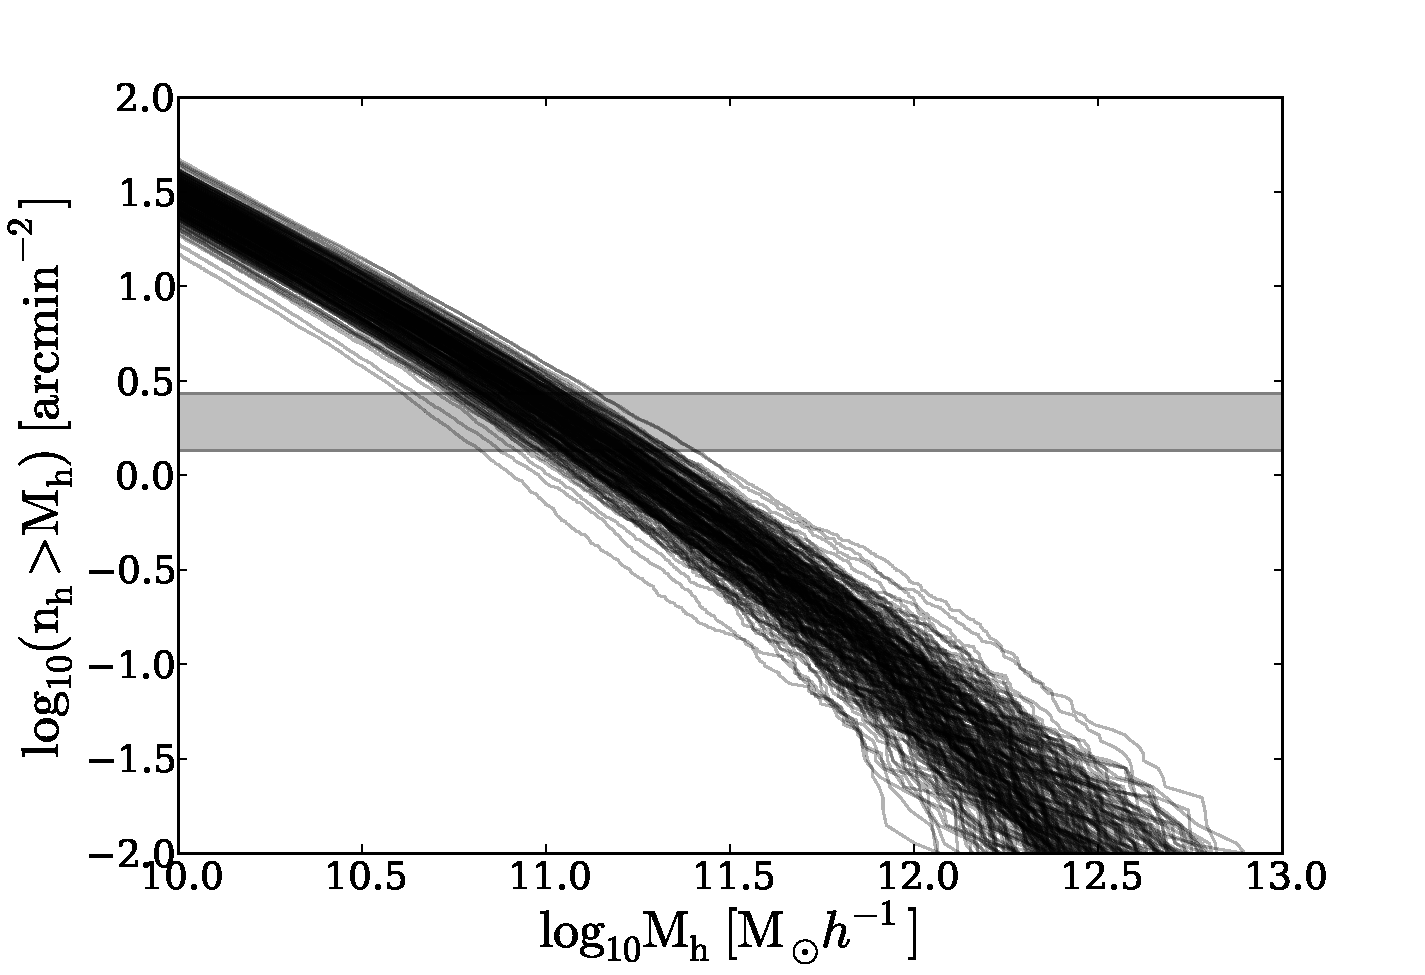
\includegraphics[width=1.00\linewidth,angle=0]{./plots/Fig1.pdf}
\caption{ \label{figure:laes_dist} Cumulative mass function of dark
  matter haloes in the $210$ sub-volumes of $46\times 35\times 41$
  $h^{-3}Mpc^{3}$. The variation in the total number of dark matter
  halos per sub-volume  evidences the effect of cosmic variance at
  such sub-volume scale. It is also appreciable the low population
  $\lesssim10^{-3}h^{2}Mpc^{-2}$ of halos with
  $log(M/M_{\odot})>12.0$}. 
\end{center} 
\end{figure}


\subsection{Dark Matter Halo Number Density}
In Figure \ref{fig:laes_dist} we present the results for  the
integrated dark matter halo surface density as a function of halos
mass. Each line corresponds to one of the 210 sub-volumes in the
Bolshoi simulation. The shadowed area indicates the surface density
values for LAEs allowed by the observations.  
 
This result allows us to better understand the expected trends for the
LAEs' preferred mass and the occupation fraction.  From this Figure we
can read which models do not have achance reproduce the
observations. Regions in the plot where the halo surface density
values are below the observational constraint correspond to high
masses halo masses. For a LAE model ${\mathcal M}$ with a minimum mass
$M_{\rm   min}> 3 \times 10^{11}$\hMsun located inthat mass range, the
surface density is too low compared with observations.   

Conversely, there are regions in the plot where the halo surface
density is always higher than the observational constraints correspond
to models ${\mathcal M}$ with a minimum mass below $M_{\rm min}<
3\times 10^{10}$\hMsun. Models with this minimum mass hava a chance
for successfuly reproducing observations if the occupation fraction
$f_{\rm occ}<1$ is tuned as to lower the halo number density down to
the observed value.    

\subsection{Kolmogorov-Smirnov Tests}

\begin{figure*}
\begin{center}
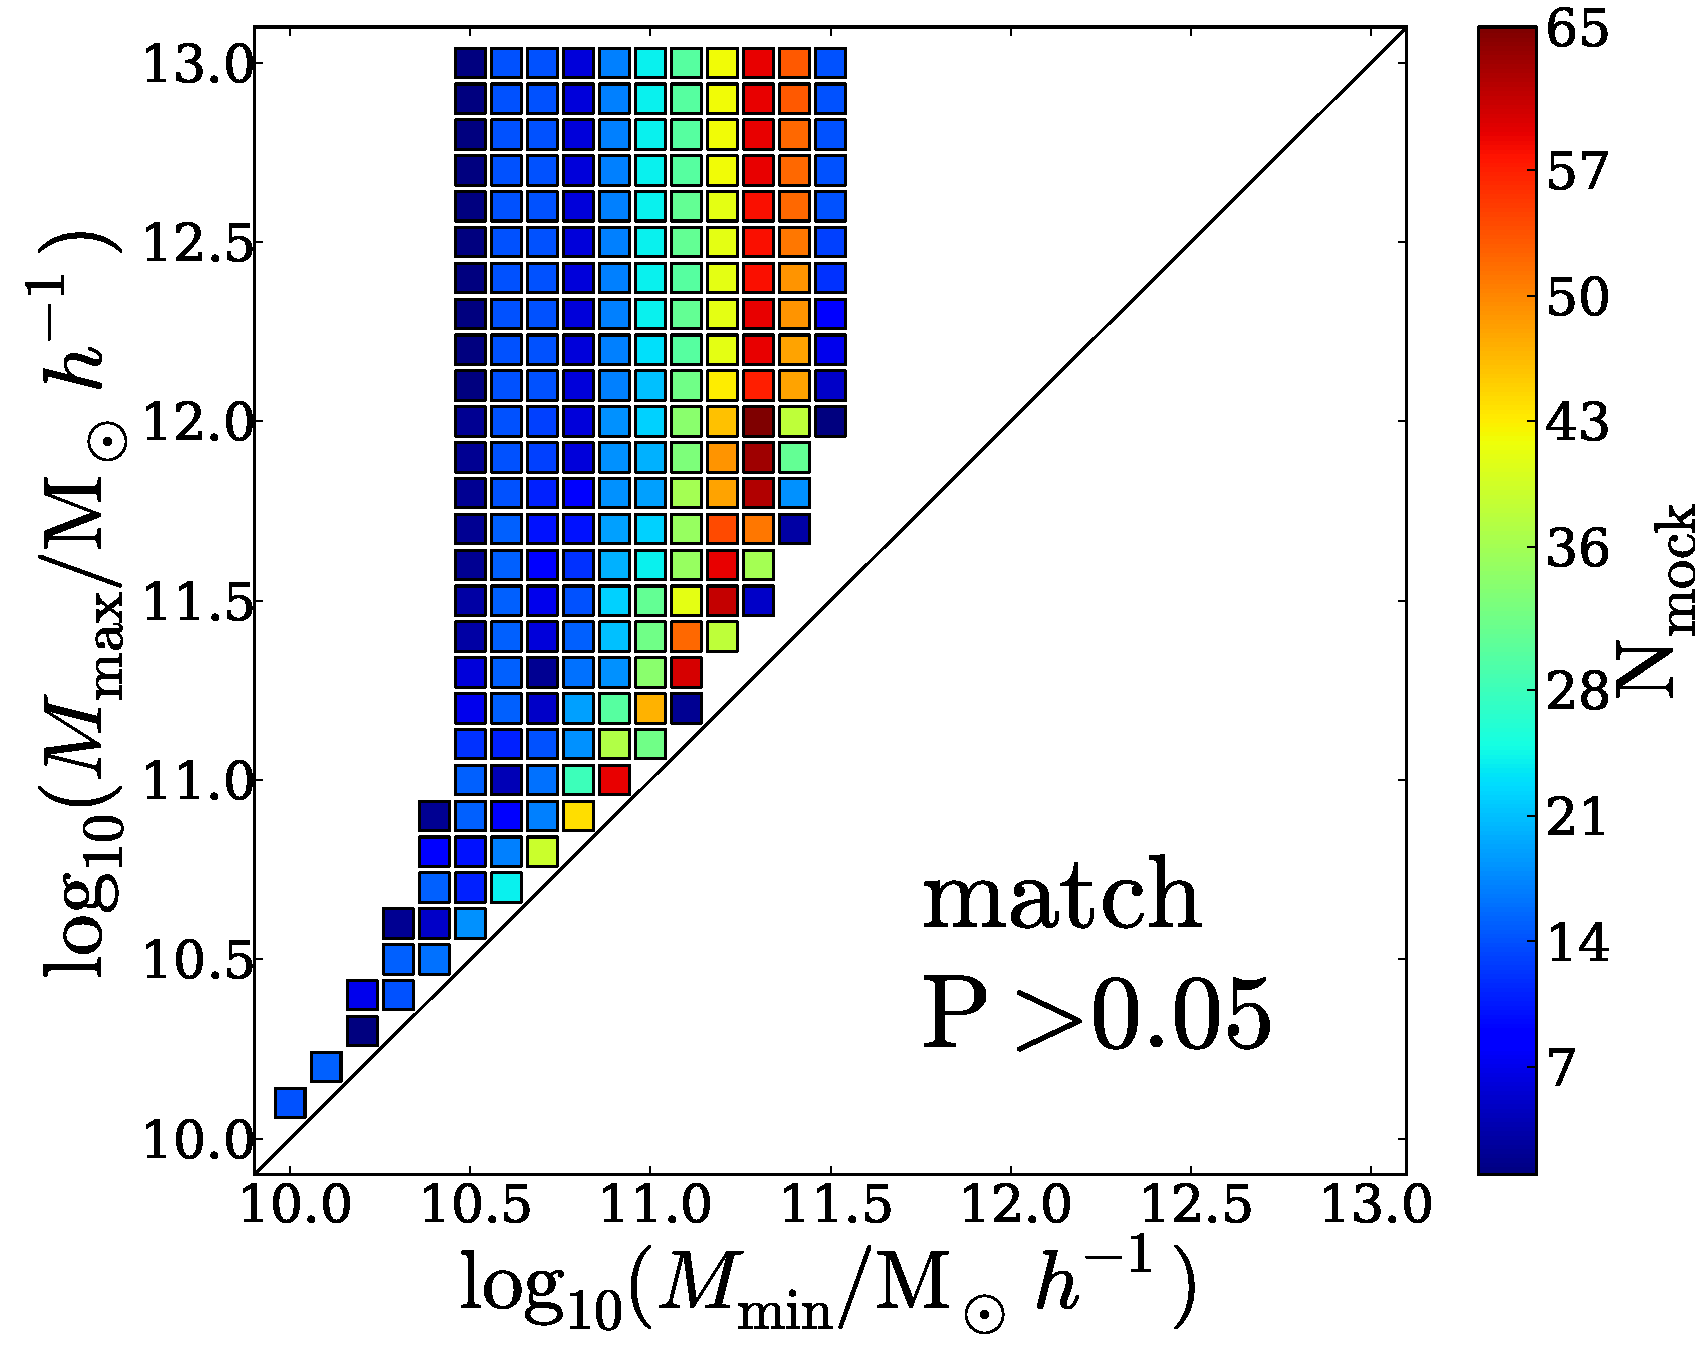
\includegraphics[width=0.46\linewidth,angle=0]{./plots/Fig2_match_P5.pdf}
\vspace{5mm}
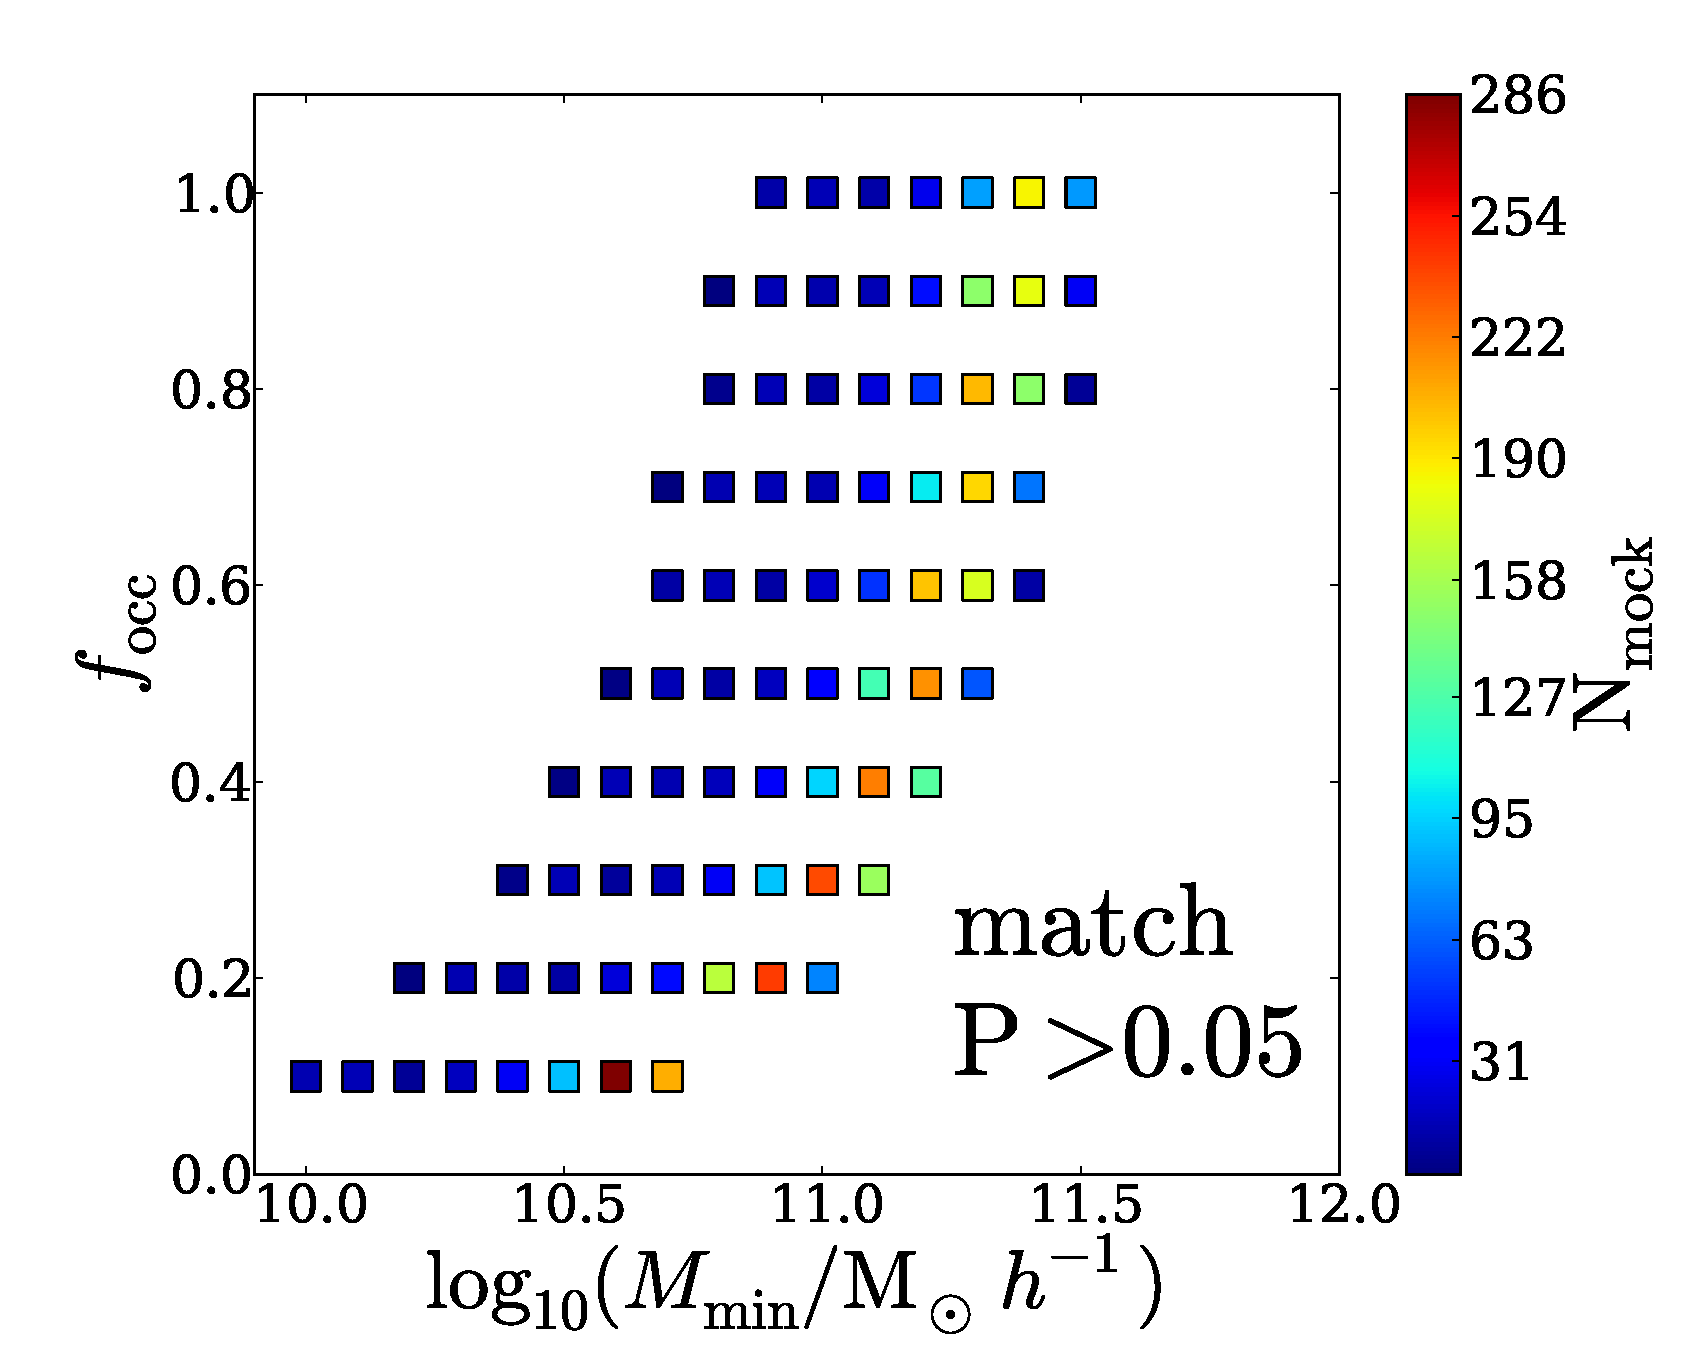
\includegraphics[width=0.49\linewidth,angle=0]{./plots/Fig3_match_P5.pdf}\\
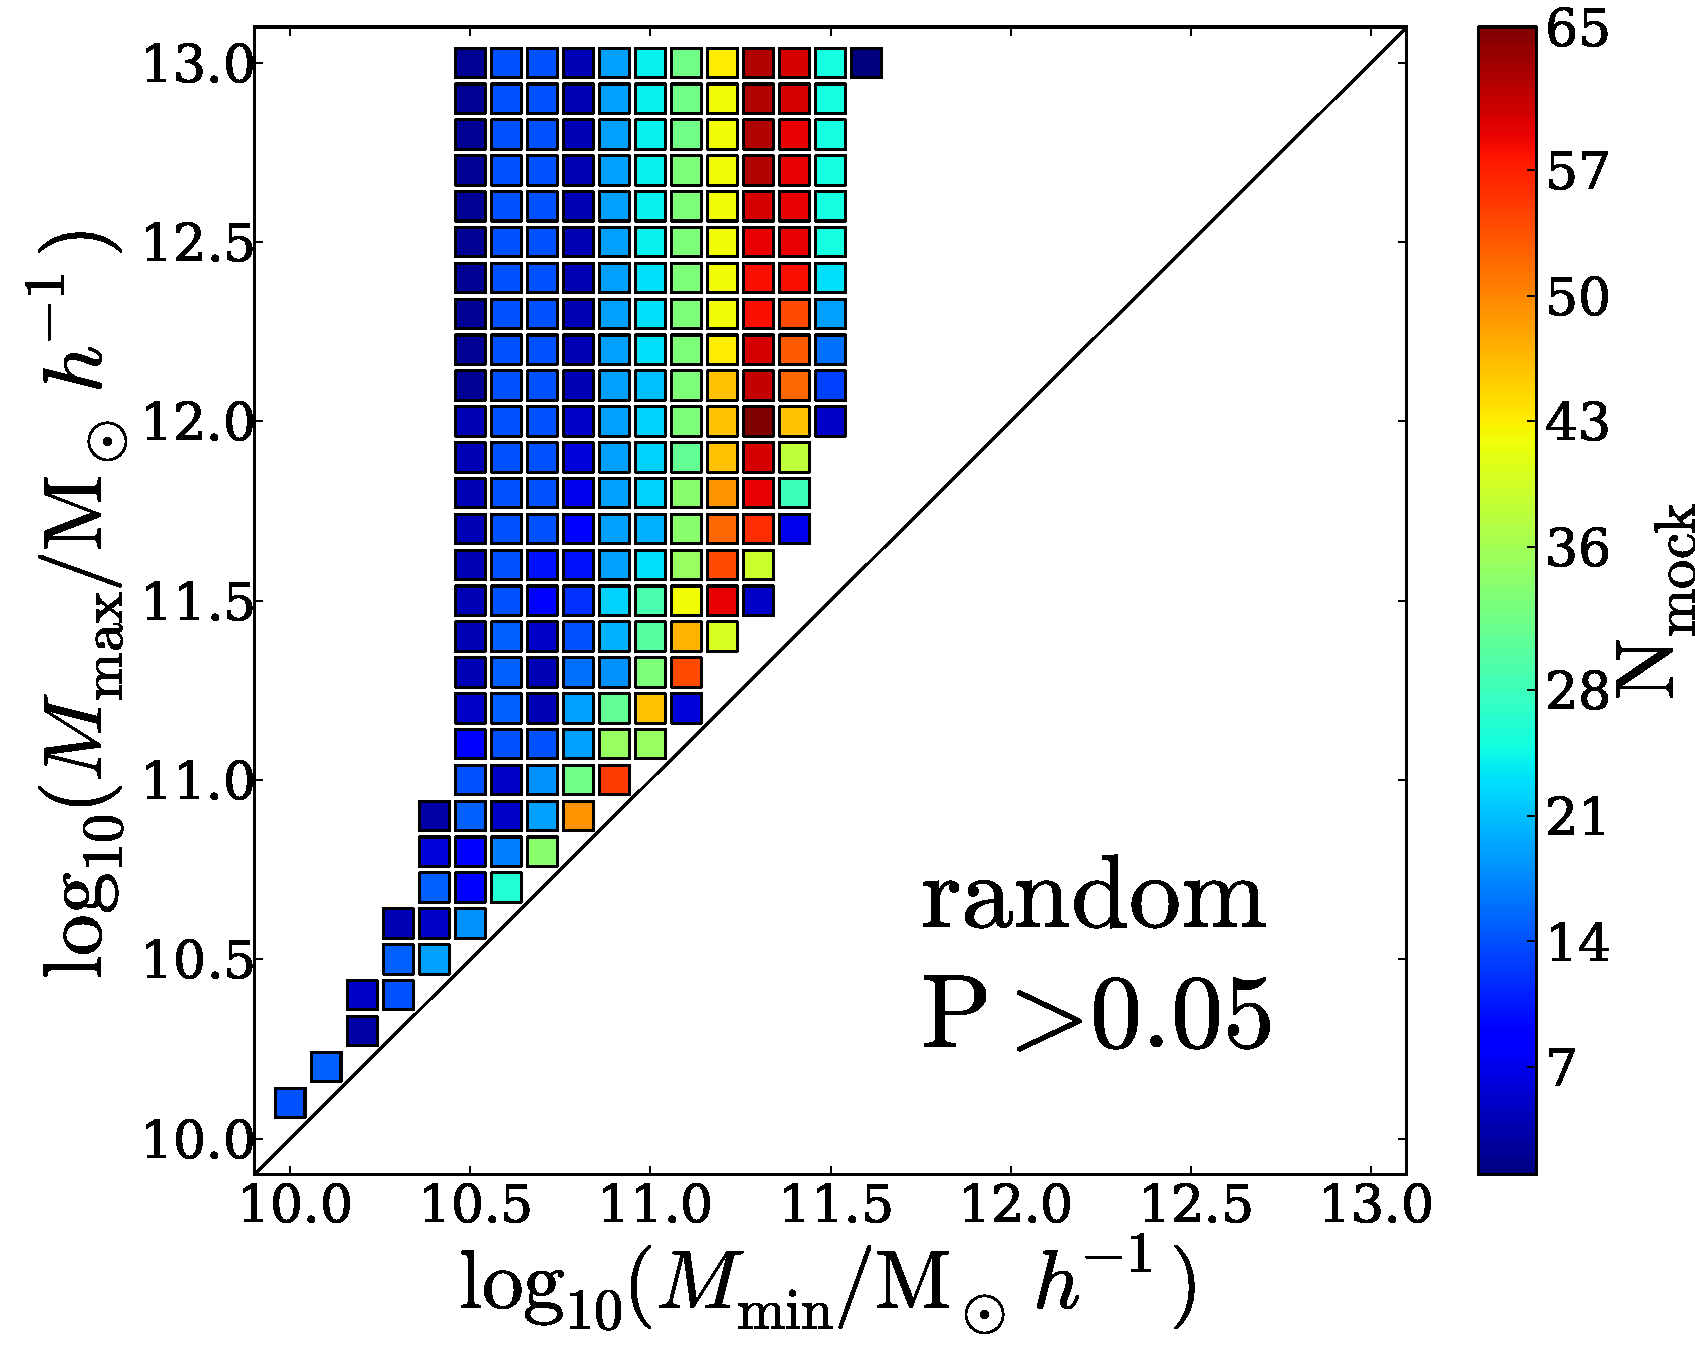
\includegraphics[width=0.46\linewidth,angle=0]{./plots/Fig2_random_P5.pdf}
\hspace{5mm}
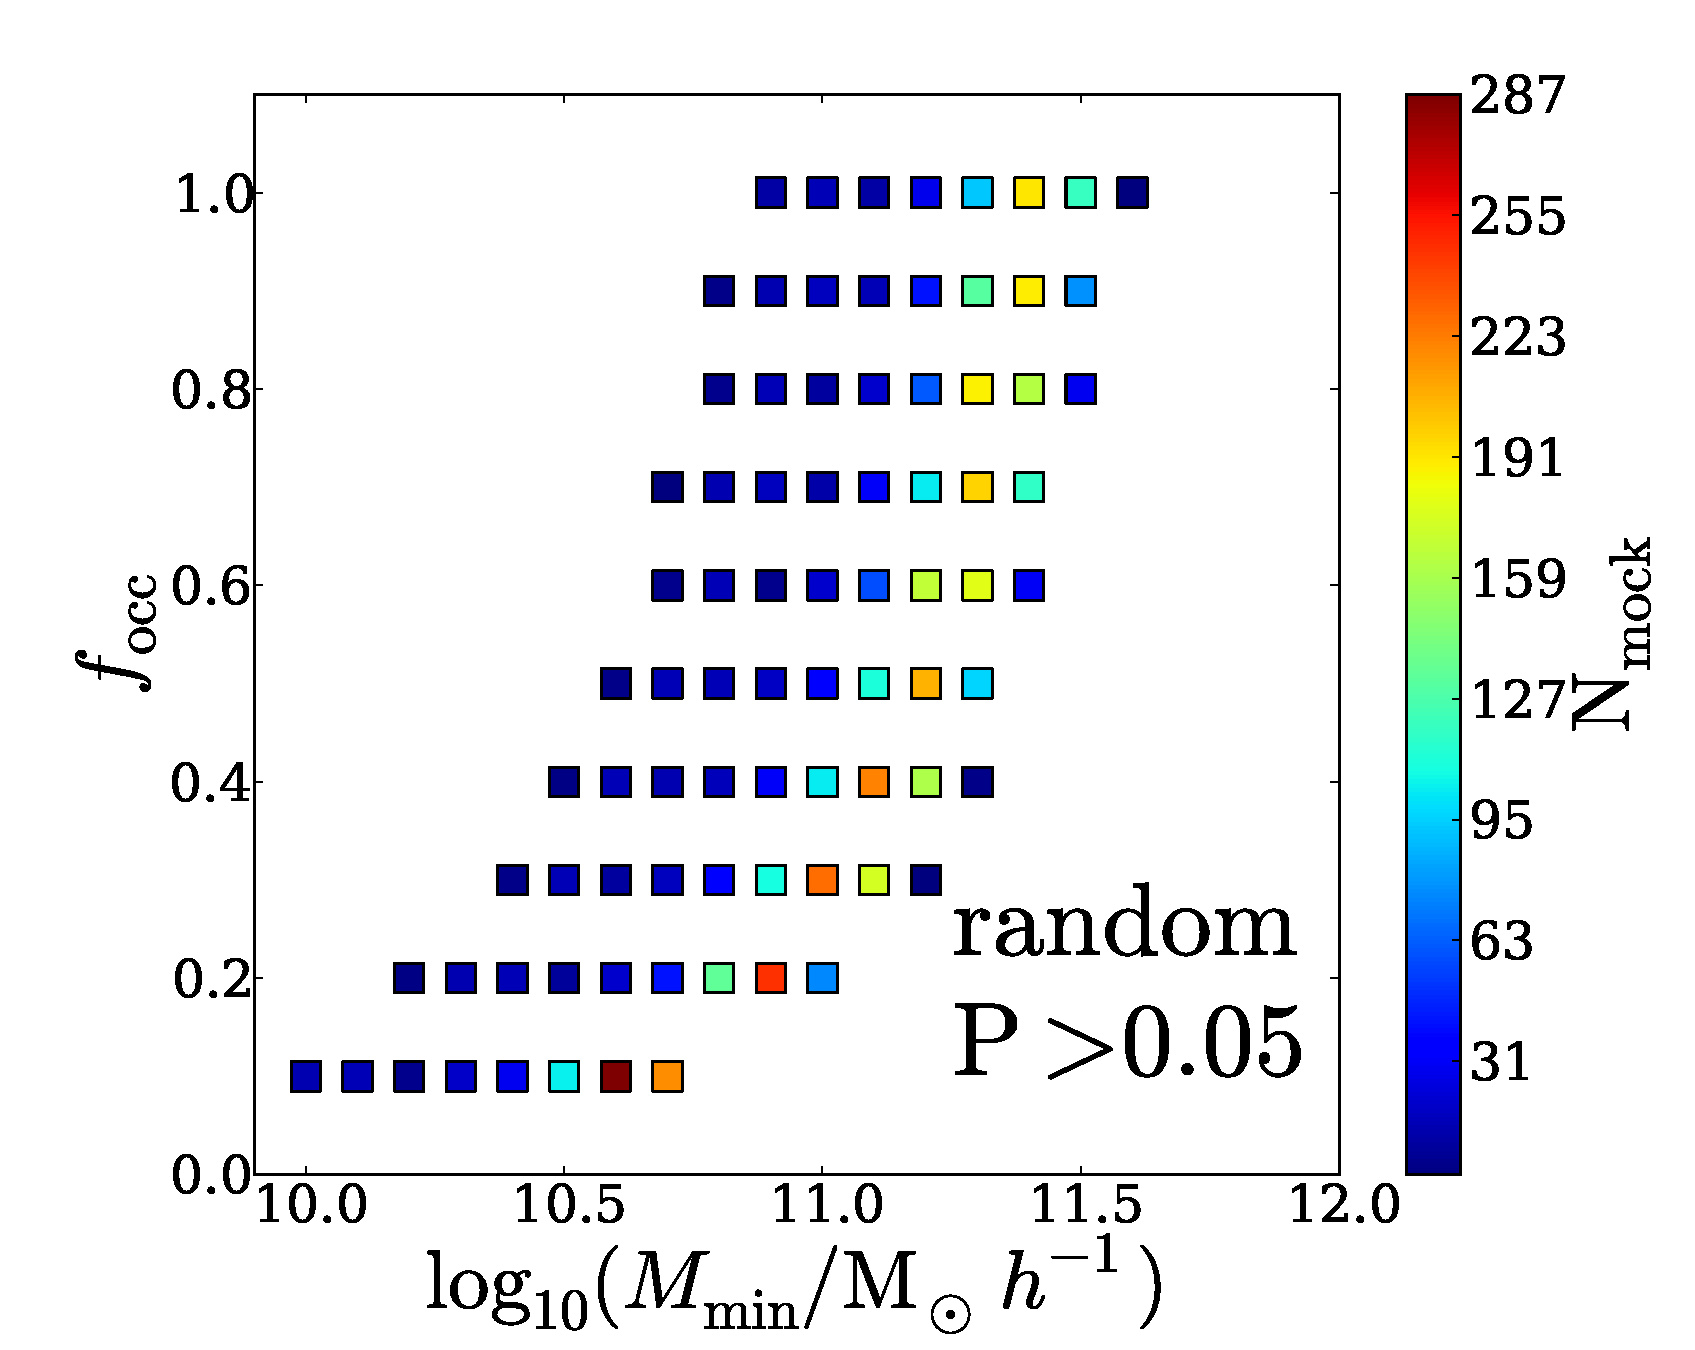
\includegraphics[width=0.49\linewidth,angle=0]{./plots/Fig3_random_P5.pdf}\\
\end{center} 
\caption{$M_{\rm min}$-$M_{\rm max}$ plane for all models with
  $P>0.05$ in the three different of grouping the mock fields. In the
  case of the {\tt match} and {\tt random} methods the  color code
  corresponds to the number of mock surveys that are found to
  be compatible with observations. For the {\tt full} method the
  colour code corresponds to the results of $100$ times the maximum $P$ value
  resulting from the KS test. \label{figure:landscape}.}  
\end{figure*}


Figure \label{figure:landscape} presents the regions in the parameter
space $M_{\rm min}$-$M_{\rm max}$ where the KS test yields values of
$P>0.05$. We consider that for those models it is not possible to rule out the null
hypothesis, namely that the number density in simulated data and the observations come
from the same parent distribution. Each panel corresponds to the three different ways of
grouping the mock fields. In the case of the methods {\tt{Match}}
and {\tt{Random}} the color code indicates the fraction of these 15
mock surveys with with $P>0.1$. The third panel shows the result for
the method {\tt{Full}}, in this case the color code correspond
to the value maximum value of $100\times P$ for a model with those
mass ranges.

These results clearly distinguish three mass regimes. In the first regime, at
high mass values, we find that LAE models with minimum mass of $M_{\rm
  min}>10^{11.5}$\hMsun are not compatible with observations. There is
a second regime for masses below $M_{\rm
  min}=3\times 10^{10}$ any values for $M_{\rm min}$ and $M_{\rm max}$
can be made compatible with observations, provided that
$f_{\rm occ}$ is fine tuned to do it. In an intermediate mass regime,
for minimum mass values $3\times 10^{10}\hMsun < M_{\rm min}< 3\times 10^{11}\hMsun$ only a
limited range of models with $M_{\rm max}$ with occupation fraction
$f_{\rm occ}\sim 1$ is able to reproduce observations. 

In these three different mass regimes the occupation monotonically
decreases as a function of the minimum halo mass $M_{\rm min}$. In
Figure XXX we show this treend in three panels following the same
correspondence as Figure XXX. From these results we interpret that the
different mass regimes that were identified correspond to best fit
models with $f_{\rm occ}\sim 1$, $0<f_{\rm occ}<1$ and $f_{\rm
  occ}\sim 0$, respectively. 

The two {\tt match} and {\tt random} methods present the highest
number of matching mock surveys in the medium mass regime. However, it
is important to keep in mind that not all the mock surveys for a
sucessful model ${\mathrm M}$ present a high value $P>0.1$, only a
modest fraction seems to be consistent with observations. This shows that the
cosmic variance is still present on the physical scales probed by
observations. This will be considered in more detail in the discussion
seccion. 

To illustrate this point, in Figure \ref{fig:mocks} we present the
results for two mock fields for the {\tt{Match}} method for a model
with the same parameters, but two extreme values for the KS test. 


Conversely there are different models where the KS test yield values of
$P\sim 1$. To illustrate the kind of success represented by these
models, we have selected these best ones in the case of the method
{\tt{MatchObs}}. Figure XXX shows in the main panel the spatial
distribution of the mock surveys, the smaller panel shows the
corresponding surface density distribution and the observational
constraint.  

In what follows we will focus our discussion on the mocks constructed
with the {\tt{Match}} and {\tt{Random}} methods. 

\subsection{Additional Constraints}

\begin{figure*}
\begin{center}
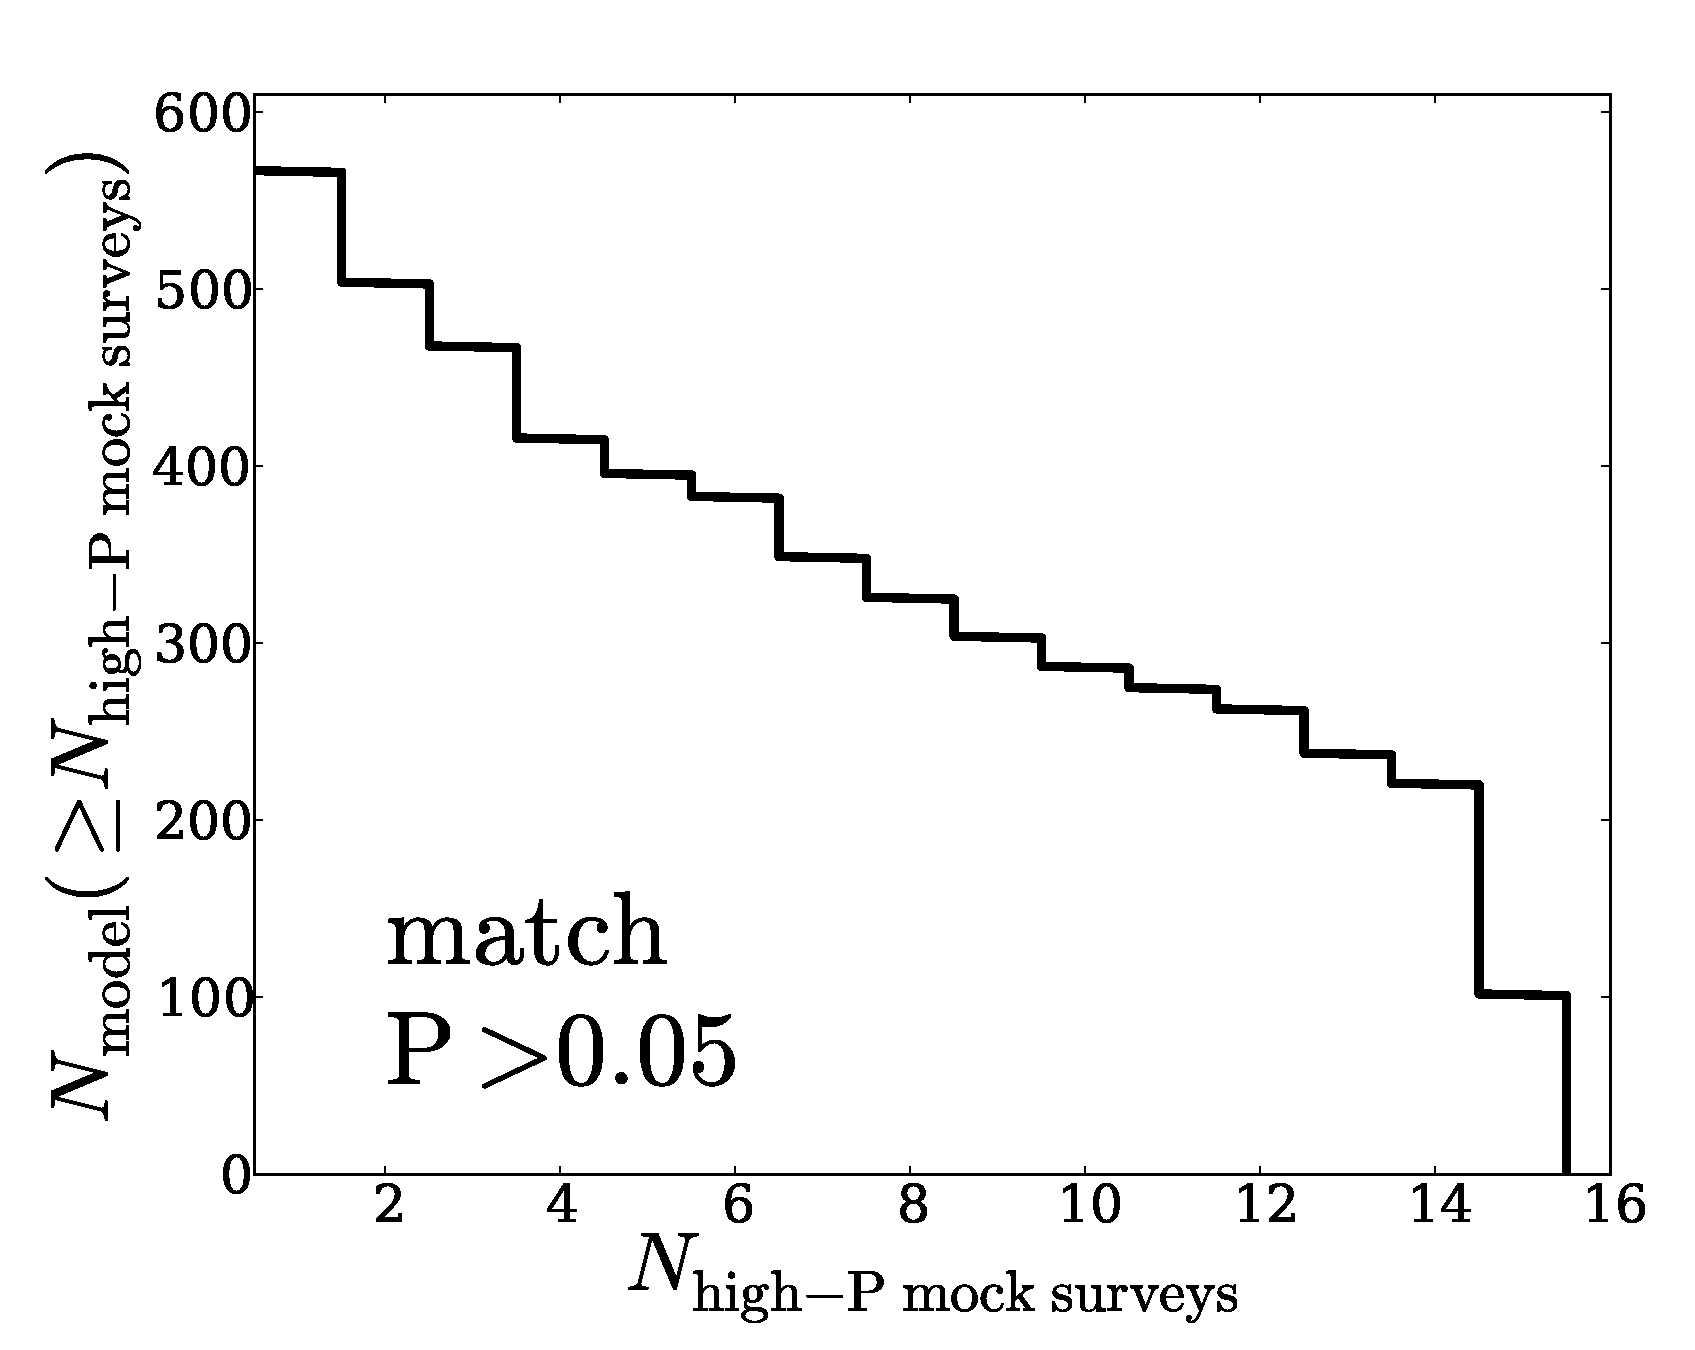
\includegraphics[width=0.46\linewidth,angle=0]{./plots/Fig4_match_P5.pdf}
\hspace{5mm}
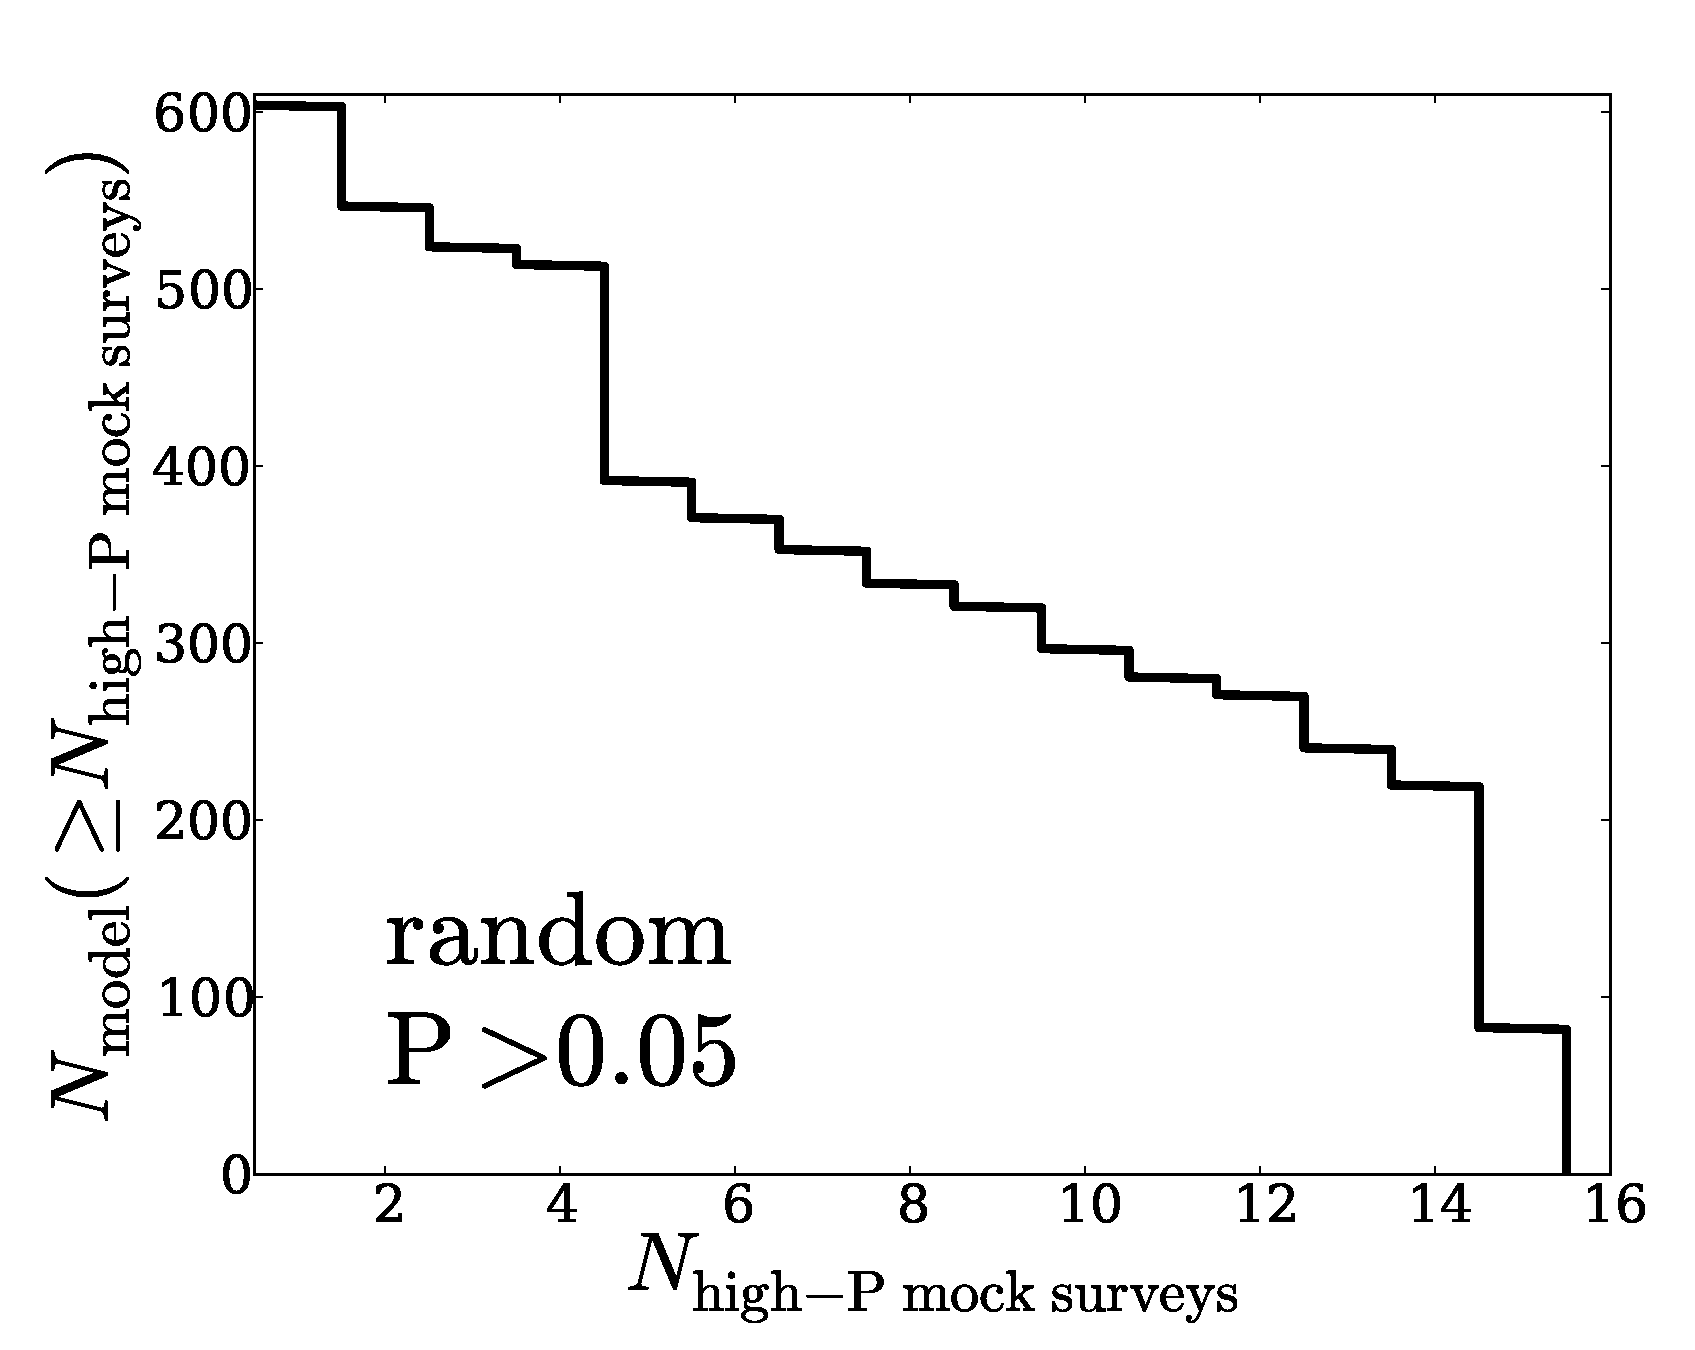
\includegraphics[width=0.46\linewidth,angle=0]{./plots/Fig4_random_P5.pdf}
\end{center} 
\caption{ Number of models with a mininium number of mock survey
  realizations that are consistent with observations.
  \label{figure:high_success_rate}.}  
\end{figure*}

The raw results of our experiments yield a prefered range for
halo masses hosting LAES bounded by a minimum mass $10^{10}\hMsun<M_{\rm
  min}<10^{11.5}\hMsun$ and without any limitation on the  maximum
mass. In this regime the average occupation fraction varies with an
approximate dependence of the kind $f_{occ}\approx 0.1 (M_{\rm
  min}/10^{10})^{XX}$. These results discard models that were
nevertheless disfavored from the very beginning based on the results
of the mass functions (see Figure 1.).  
 

In this section we consider three different ways to impose
tighter constraints on this mass range by making use of the results we
have derived so far together with additional statistical and
astrophysical constraints. In the first constraint we select the
models where all the mock surveys present KS-test values consistent
with observations. The second constraints uses recent observational
results on the average occupation fraction for LAEs at high-z. The
third exploits the information in the Angular Correlation Function
(ACF).  

\subsubsection{Models with the highest success rates}

For each model there are 15 different mock survey realizations. In the
previous section we presented the models that had at least one (1)
mock survey realization with $P>0.05$.

In Figure \ref{figure:high_success_rate} we show the number of models
that have at least $n$ realizations with $P>0.05$ for the {\texttt
  match} and {\texttt random} methods.  This shows that there are
around $550$ to $600$ different models that have at leaset one mock
survey realization consistent with observations. At the other extreme,
there are $80$ to $100$ models with all the 15 realizations with
$P>0.05$. Here we focuse on the latter models. The best models
represent $\sim 15\%$ of the number of initially considered good
models. 

In Figure XX we present the locii of these models in the parameter
space $M_{\rm min}-M_{\rm max}$ and $M_{\rm min}-f_{\rm occ}$. In
Figure XX we show the spatial distribution for two mock surveys
corresponding to one of such models. 




\subsubsection{Observational constraints on the occupation fraction}

We now impose a different restriction using the observational results
by \cite{Hayes2010}. These authors constrained the value of $f_{\rm
  occ}$ at $z=2.2$ to be $f_{\rm occ}=0.10$. This estimation was based
on blind surveys of the H$\alpha$ and Lyman alpha line with the European Southern
Observatorio (ESO) Very Large Telescope (VLT). Using corrections by
extinction to obtain an estimate for the intrinsic H$\alpha$
luminosity, and using values for the theoretical expectation of the
ratio Lyman$\alpha$/H$\alpha$ they derive an bulk escape fraction for
the Lyman$\alpha$ radiation of $f_{\rm esc}=(5.3\pm 3.8)\%$ or $f_{\rm
esc}=(10.7\pm 2.8)$ if a different dust correction is used. The
authors show that the luminosity function for LAEs at $z=2.2$ is
consistent with the escape fraction being constant for every galaxy
regardless of its luminosity. From this results they derive that
almost $90\%$ of the star forming galaxies emit insufficient
Lyman-alpha to be detected, effectively setting the occupation
fraction to be $f_{\rm occ}=0.10$.  

For the cosmological parameters used in this \documentname the age of
the universe between $z=3.1$ and $z=2.2$ has changed by $\sim 1$
Gyr. We assume that the physical conditions that determine the escape
fraction $f_{\rm esc}$ and the occupation fraction $f_{\rm  occ}$
remain constant over that time scale. This assumption allows us to
further pick models that have an occupation fraction of $f_{\rm
  occ}=0.10$. Under this selection only $18$ models can
beselected. Considering an occupation fraction $f_{\rm occ}=0.20$
another $39$ models can beconsidered. This constraint help us to
select $\sim 10\%$ of theoriginal models that were considered as
consistent with observations in the previous section. 

Figure XX shows the prefered models in the planes $M_{\rm min}-M_{\rm
  max}$ and $M_{\rm min}-f_{\rm occ}$ for the {\tt match} and {\tt
  random} methods. The list for the model parameters is found in the
appendix in Table XX.  

In terms of the constraints done in the previous sub-section, we find
that the models in this region of parameter space have an average
number of XX mock catalogs consistent with observations. 


\begin{figure*}
\begin{center}
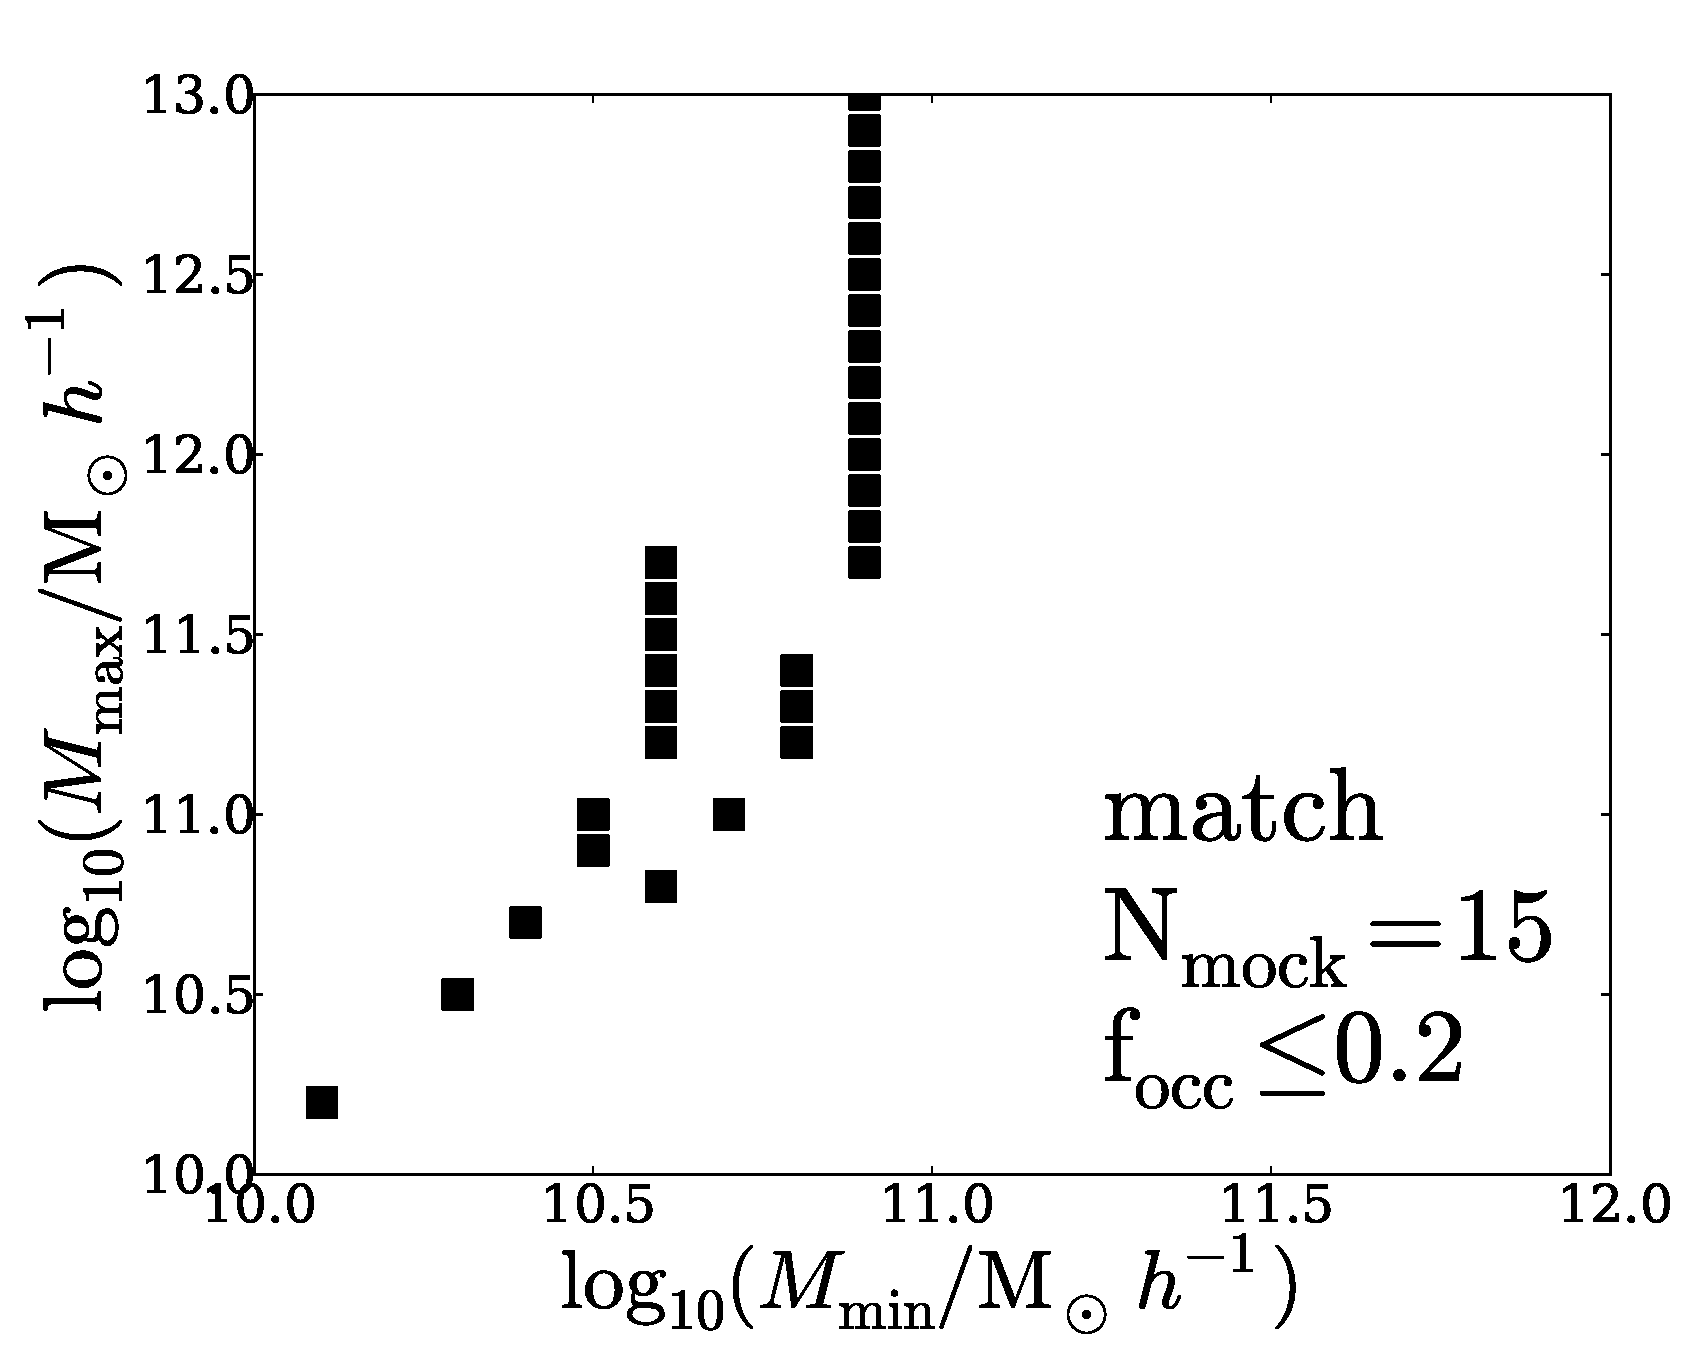
\includegraphics[width=0.46\linewidth,angle=0]{./plots/Fig5_match_mass_mock_and_f_occ.pdf}
\hspace{5mm}
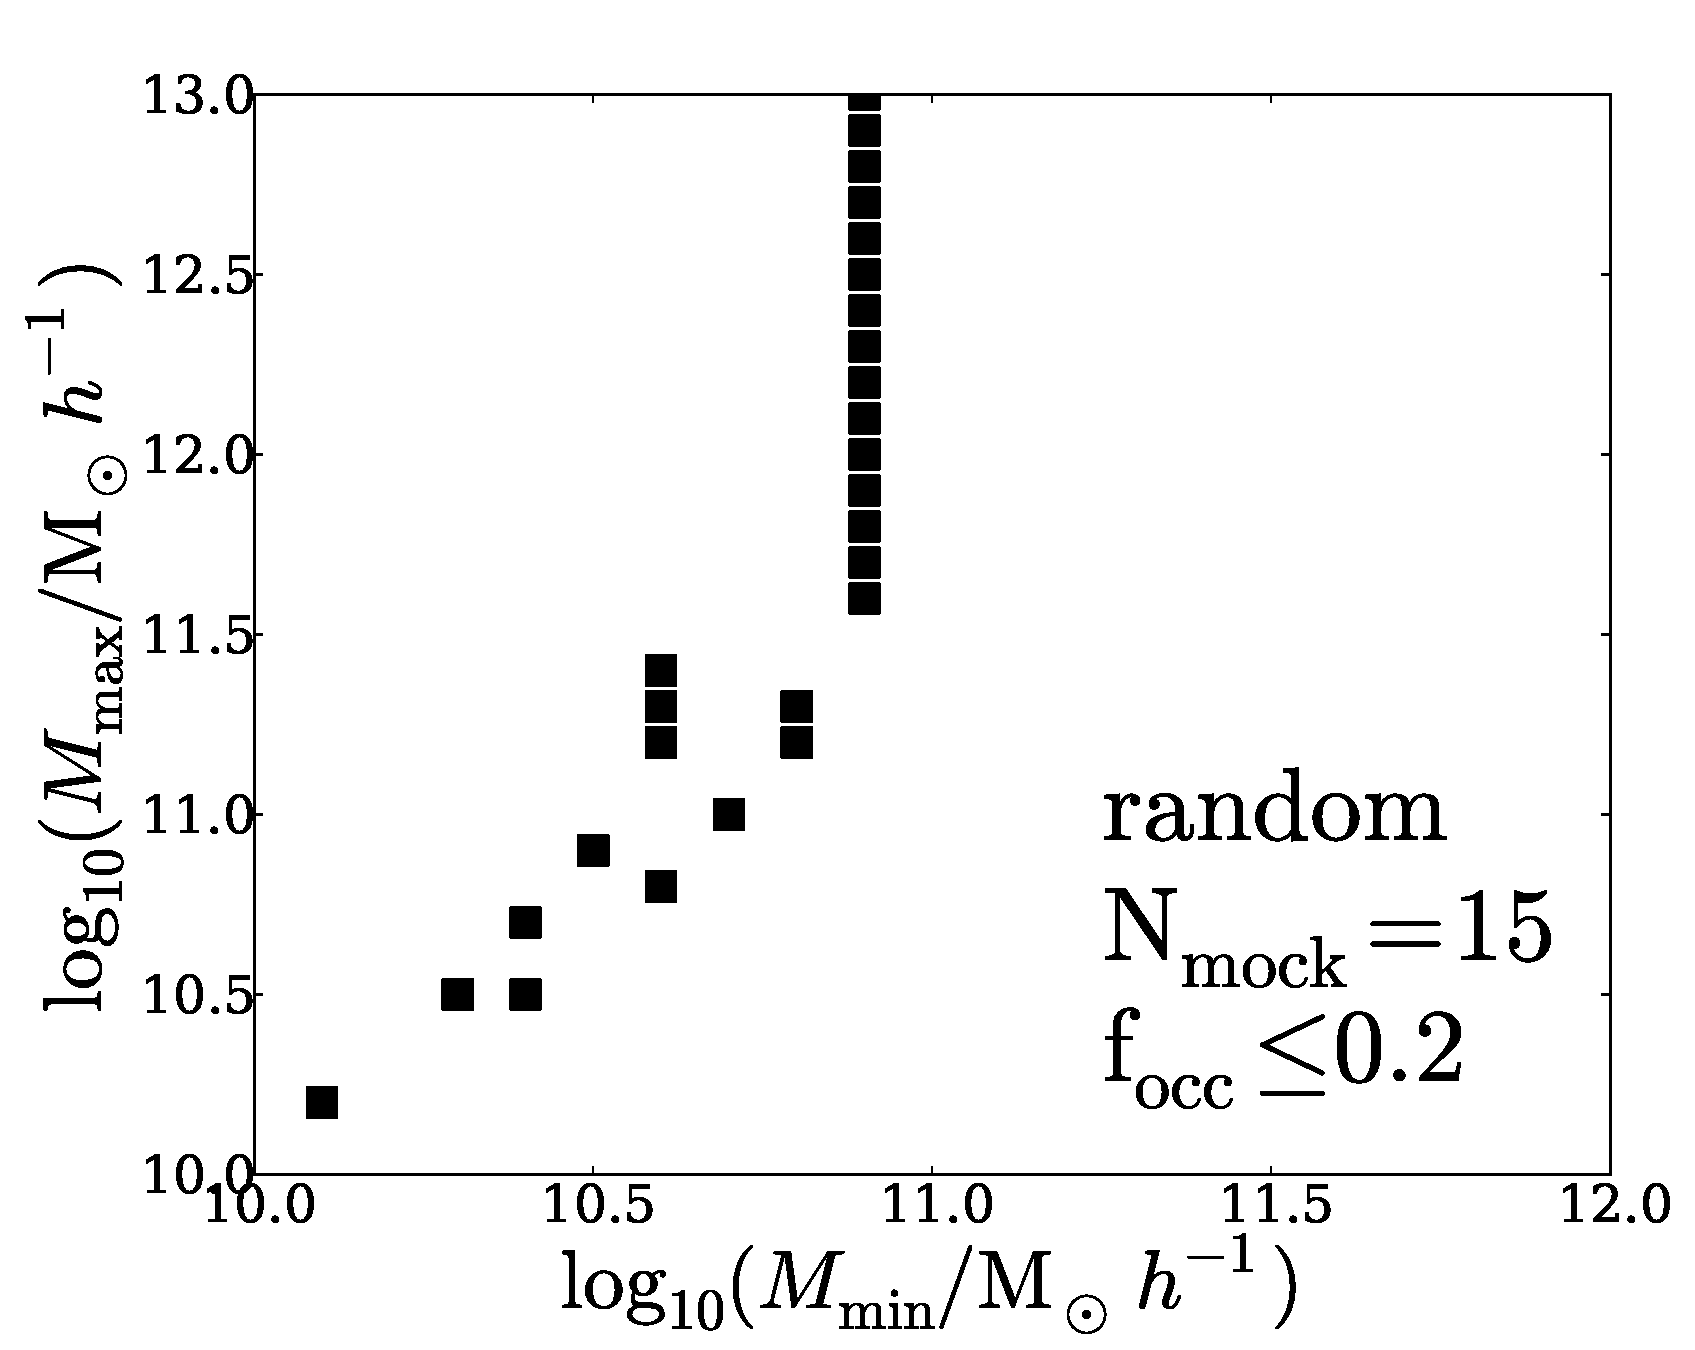
\includegraphics[width=0.46\linewidth,angle=0]{./plots/Fig5_random_mass_mock_and_f_occ.pdf}
\end{center} 
\caption{Favored models when the constraints on the maximal number of
  consistent mocks and the observational constrain on the occupation
  fraction are included.
  \label{figure:mock_and_f_occ}}  
\end{figure*}



\subsubsection{Constraints from the Angular Correlation Function}

We calculate the mean angular correlation function (ACF) only for the
models that showed that all of the 15 mock surveys are consistent
at the $P>0.05$ level with observations. The ACF is computed only the
denseset subfield in all the 15 mock surveys corresponding to the
SSA22 region. These results are compared against the observations
reported by Hayashino et al in 2004 over the same region, which were
also performed on the densest field.   

Figure \ref{figure:correlation_match} (match) and Figure
\ref{figure:correlation_random} (random) present such comparison.  The
error bars in these figures represent the standard deviation of the
ACF over all the sub-fields.  In general, we observe that the standard
deviation of the computed ACF in the subfields increases with
$M_{min}$ following the same trend as in Figure
\ref{figure:laes_dist}, as a direct consequence of cosmic variance.  


The comparison between the simulated and observed ACFs is also done using a
$R^2$ statistic which includes the information on measurement uncertainties

\begin{equation}
R^{2} = \sum_{\theta_i} \frac{(\xi_{\rm obs}(\theta_i) - \xi_{\rm
    sim}(\theta_i))^2}{\sigma_{\rm obs}^2(\theta_i) + \sigma_{\rm
    sim}^2({\theta_i})}, 
\end{equation}

where the sum is done over all the angle values $\theta_i$ where the
ACF has been computed. In Figure XX we plot the integrated
distributions for this $R^{2}$ statistics 

Given that the ACF reported by Hayashino et al en 2004 is taken over
the densest  field oserved in the SSA22 region by  Yamada et el in
2012 it is expected that the predicted ACF in the SSA22 region should
reproduce this observation. In the  left panel of figure
\ref{figure:correlation_match} we can see the predicted ACFs  an their
corresponding standard deviation over the seven fields that mock the
SSA22  region. It can be seen that the model with $M_min=10.6$ seems
to better reproduce the  Hayashino's ACF and that the corresponding
field is in fact an overdense field in the SSA22 region covered by
Yamada et al. 

From these tests we conclude that the ACF on small fields does not
provide additional constraints to further select models for halos
hosting LAEs. The reason is that cosmic variance is large and the
statistical uncertainties on the ACF render almost any model
compatible with the observational constraints. 

We also present the ACF in the case of the full SSA22
region which has been homogeneously observed by \citep{Yamada2012}. To
this date the observational ACF has not been reported in the
litereature, therefore our calculations can be considered as
predictions. 

In Figure X we present the results for the models. The full list of
these correlation functions can be found in the the data repository
for this paper in \verb"github". 

We also present the results for the angular correlation function in
therms of the correlation lenght obtained by fitting the following
function

\begin{equation}
\xi(r) = \left(\frac{r}{r_{0}}\right)^{-\gamma}
\end{equation}

The results are shown in Figure in a $r_{0}-\gamma$ plane where the
average and standard deviation for each mock are shown in comparison
with the result derived from observations. 


\begin{figure*}
\begin{center}
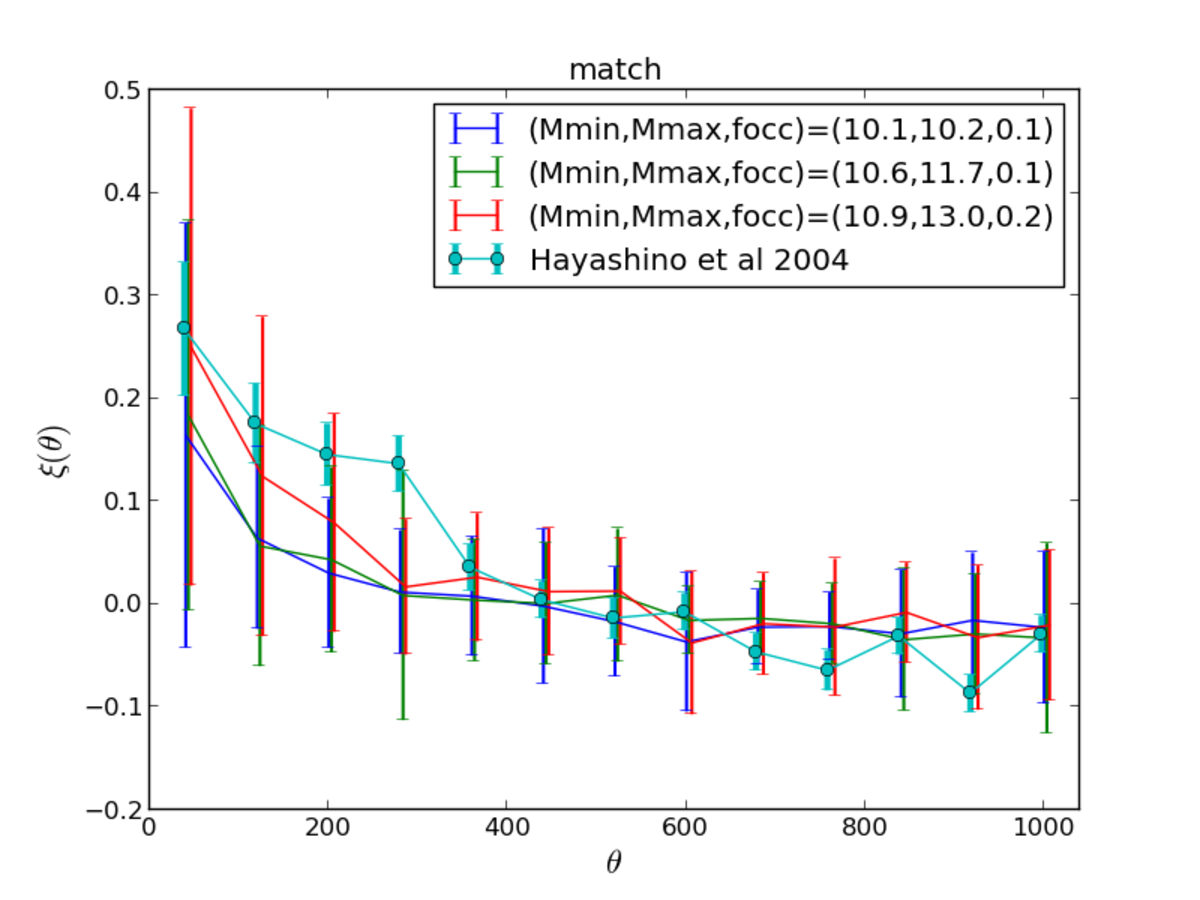
\includegraphics[width=0.46\linewidth,angle=0]{./plots/match_large_correlation_selected_models.pdf}
\hspace{5mm}
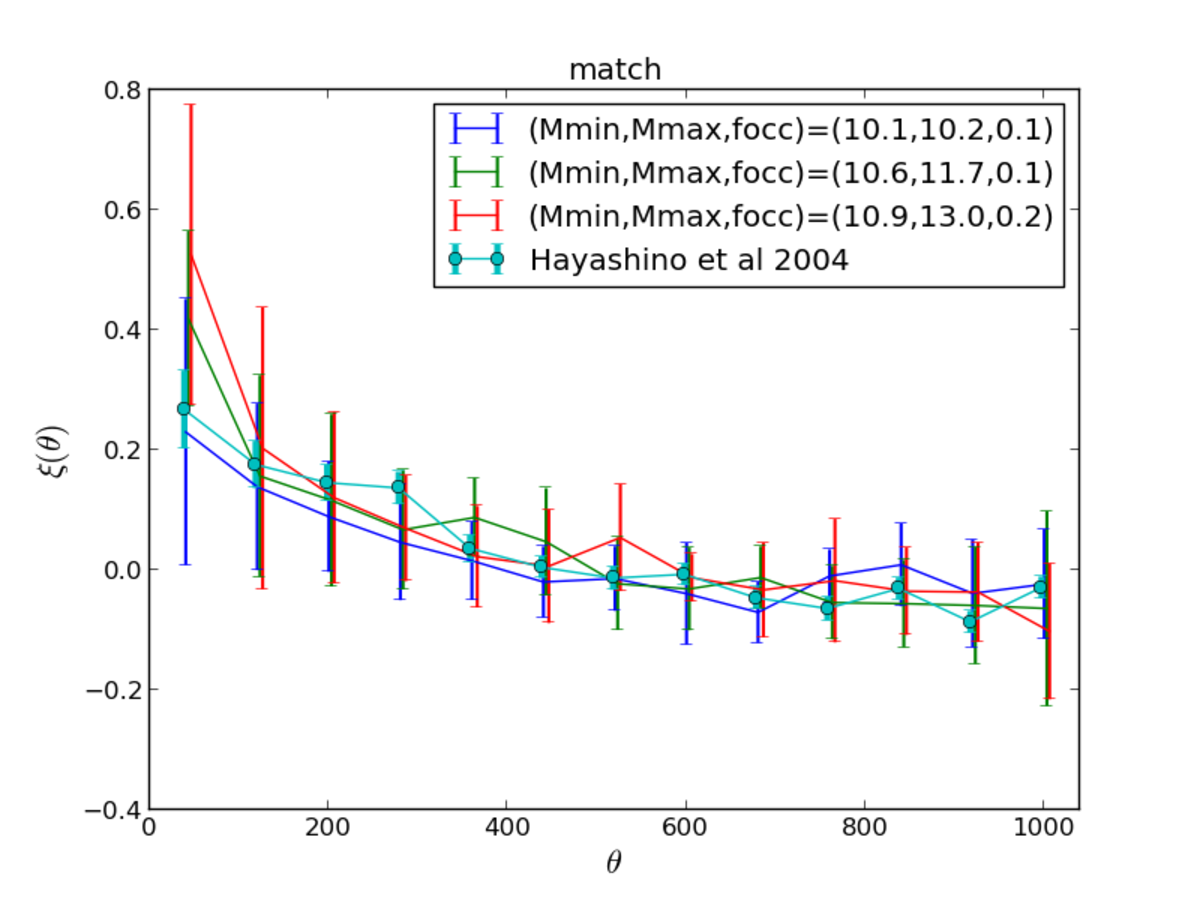
\includegraphics[width=0.46\linewidth,angle=0]{./plots/match_full_correlation_selected_models.pdf}
\end{center} f
\caption{ mean ACFs   and their correponding standard deviation (error
  bars)  of some selected models in different mass ranges over the 7
  subfields  f the SSA22 field (left) and the entire 12 field sample
  (rigth) using thematch
  configuration. \label{figure:correlation_match} }  
  \end{figure*}

\begin{figure*}
\begin{center}
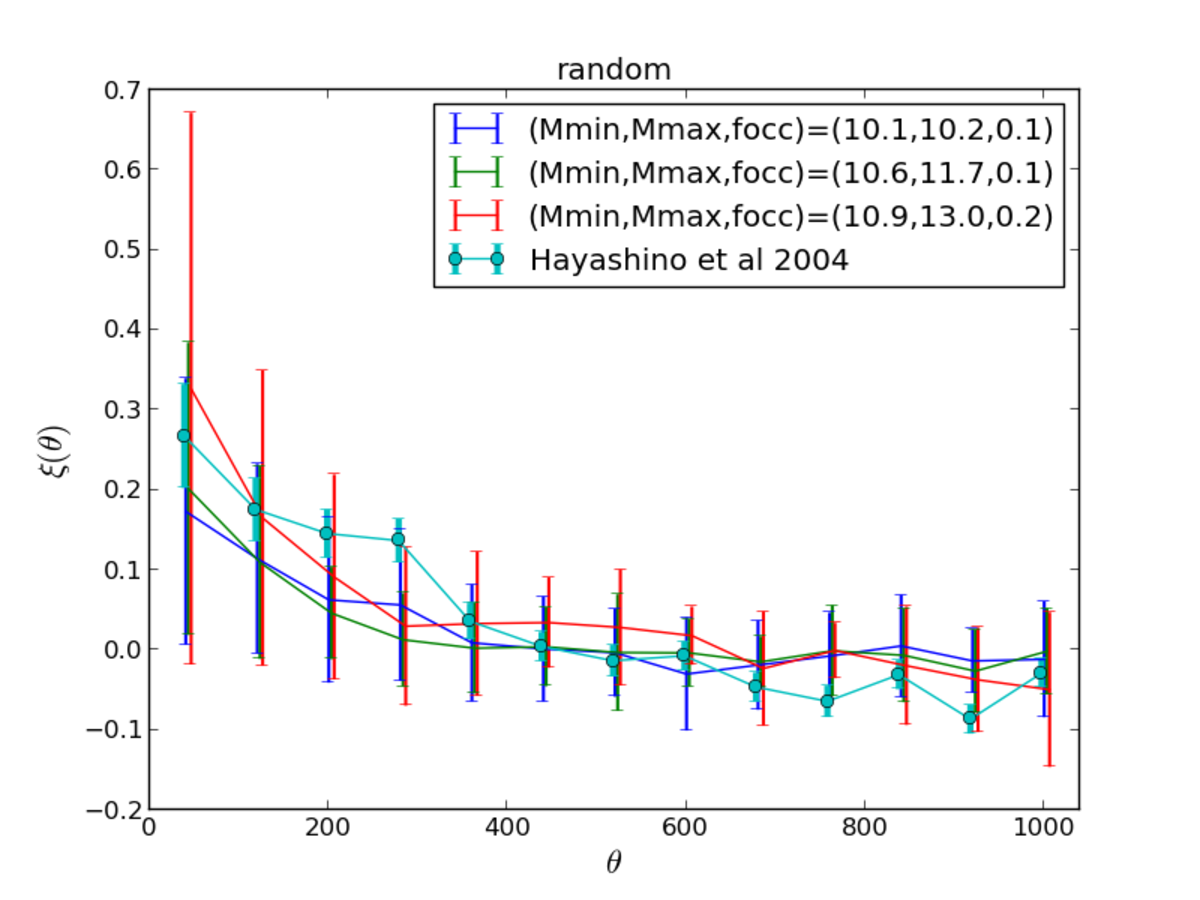
\includegraphics[width=0.46\linewidth,angle=0]{./plots/random_large_correlation_selected_models.pdf}
\hspace{5mm}
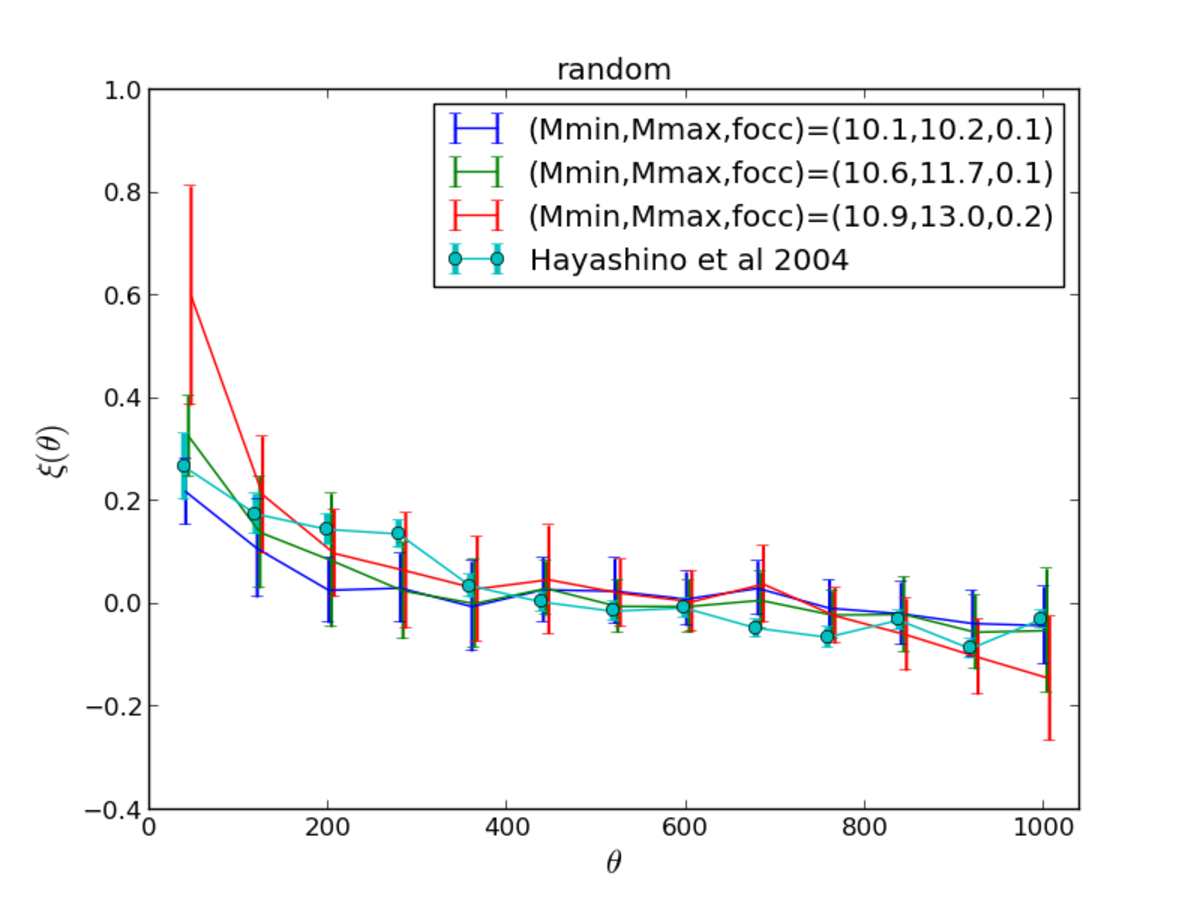
\includegraphics[width=0.46\linewidth,angle=0]{./plots/random_full_correlation_selected_models.pdf}
\end{center} 
\caption{ mean ACFs   and their correponding standard deviation (error
  bars)  of some selected models in different mass ranges over the 7
  subfields of the SSA22 field (left) and the entire 12 field sample
  (rigth) using the  random
  configuration. \label{figure:correlation_random} }  
  
\end{figure*}

\section{Discussion}



\begin{figure*}
\begin{center}
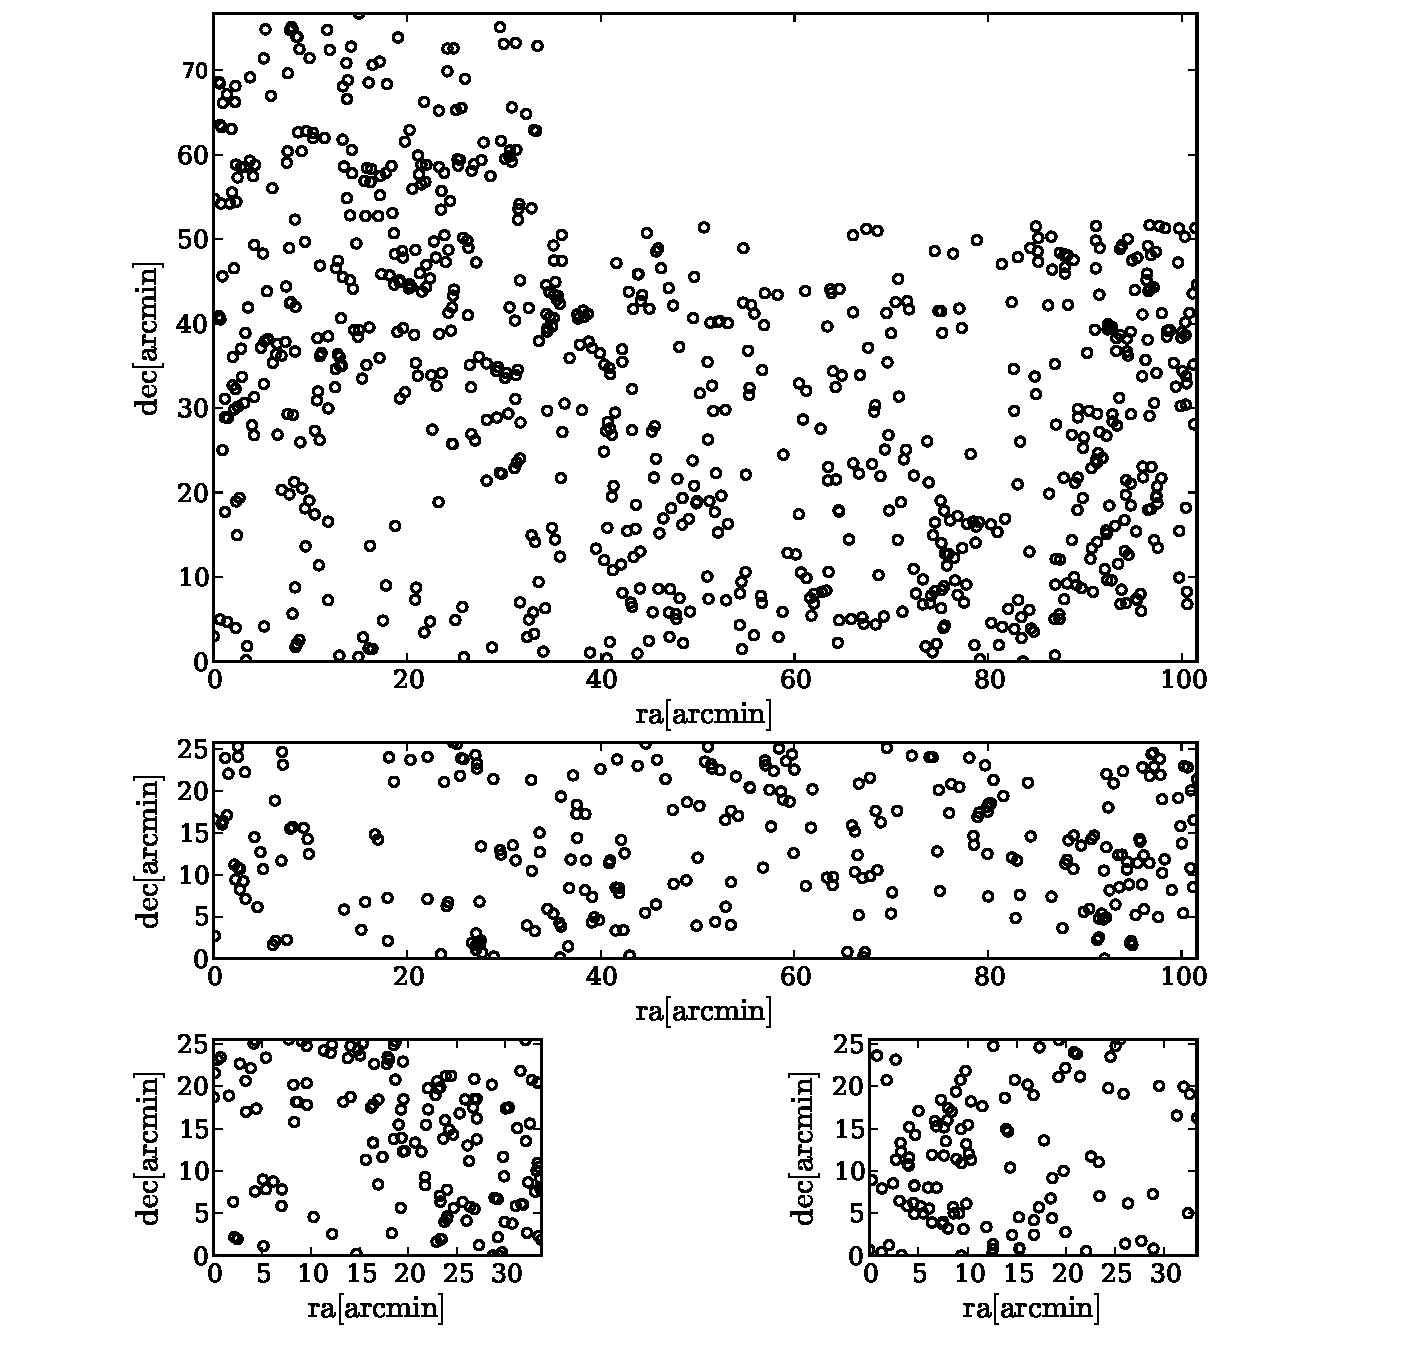
\includegraphics[width=0.49\linewidth,angle=0]{./plots/mytest.pdf}
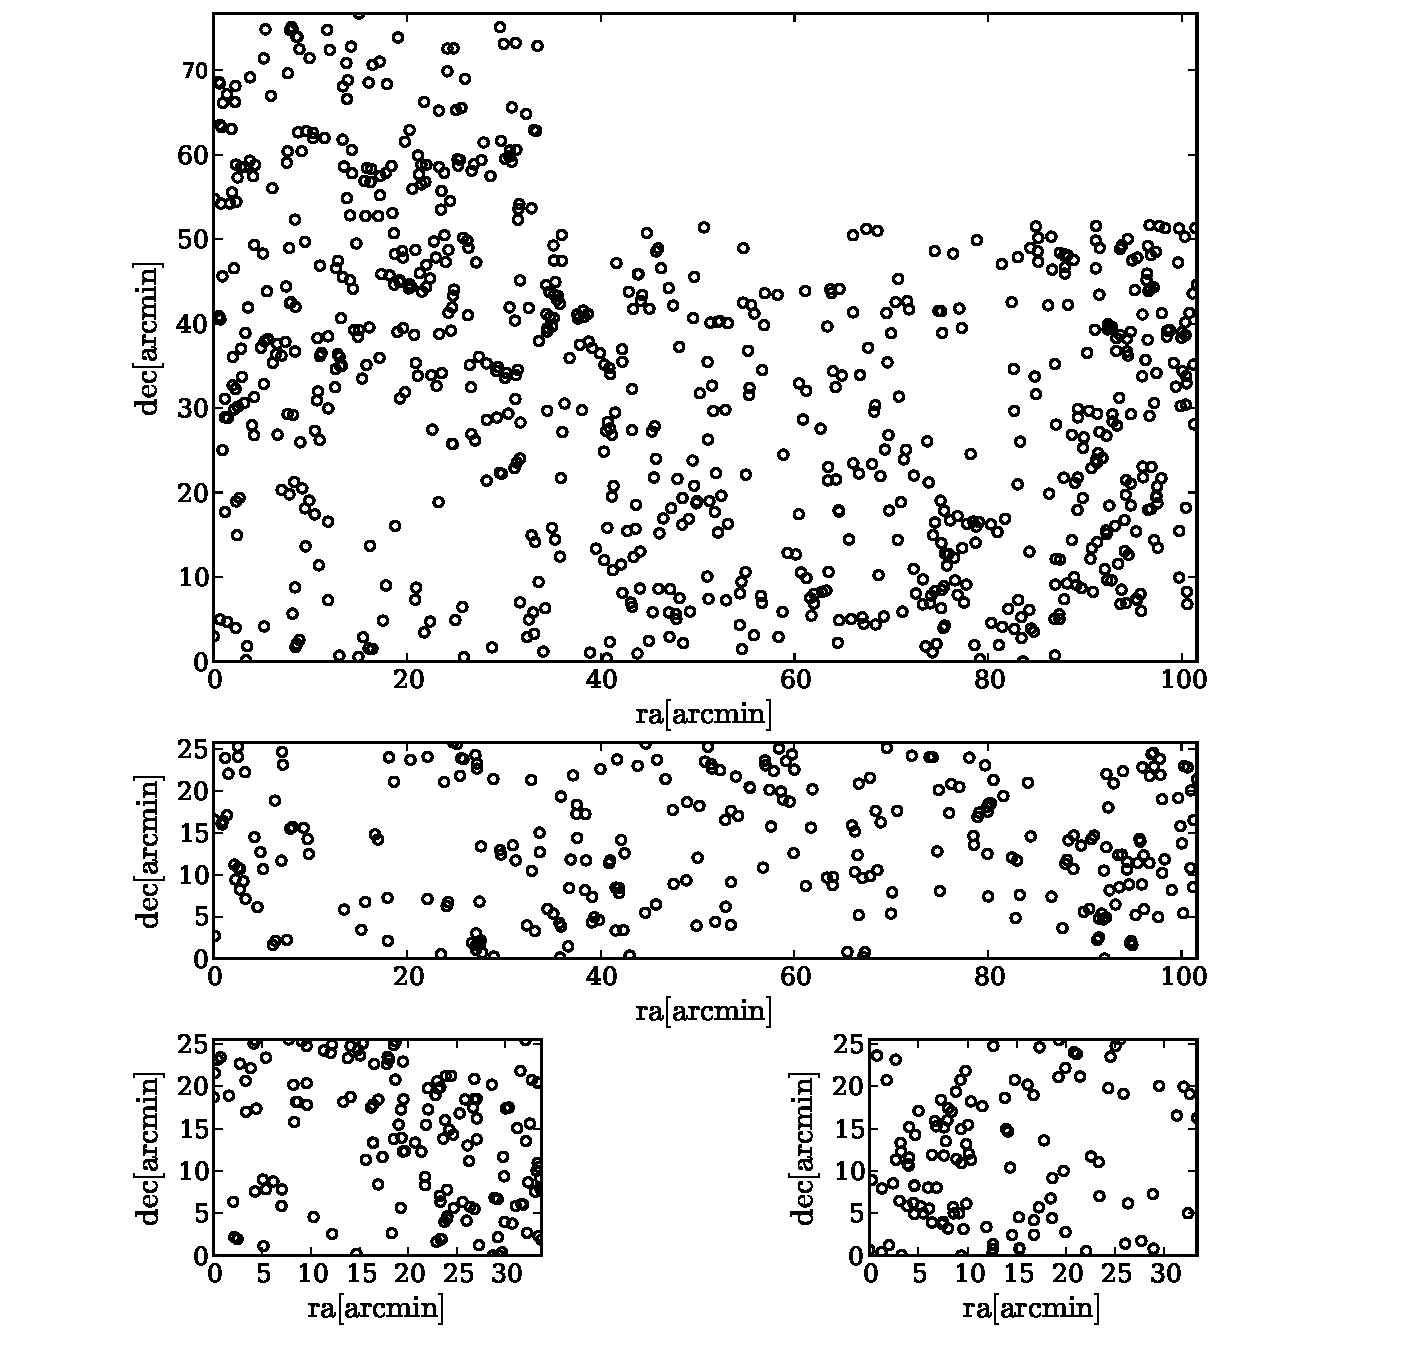
\includegraphics[width=0.49\linewidth,angle=0]{./plots/mytest.pdf}
\end{center} 
\caption{Spatial distribution for two mocks corresponding to the model
  $M_{\rm min}=$, $M_{\rm max}=$ and $f_{\rm occ}=$. All the 15
  different mock  surveys for this model in the {\texttt match}
  configuration are consistent with observations at the $P>0.05$
  level. The full data for all the mocks can be found in the github
  repository for this paper.
  \label{figure:spatial_distro}.}
\end{figure*}


When we include the tightest constraints on the mock catalogs, we find
that there are 30 set of parameters of our model, out of the original
90000 initial models, that are consistent with the observational
constraints at redshift $3.1$: the distribution of the number density,
the inferred values for the average occupation fraction. The
consistency with the angular correlation, in terms of the $\chi^2$
statistics did not help to discard any additional models with a
significant degree of confidence. 


These 30 models can be classified into two families of the same
size. The first, where the range $M_{\rm min}-M_{\rm max}$ is narrow,
typically of less than $<1.0$ dex. While in the second familiy the
extent $>1.0$ dex. In the first case the minimum halo mass is found to
be in a wide range $10^{10}\hMsun <M_{\rm min}< 10^{11.5}\hMsun$ while
in the second case, only models with $M_{\rm min}\sim 10^{10.9}\hMsun$
are compatible with the observational contraints. In what follows we
discuss the implications of the existence of these two families of
models.  

\subsection{Implications for galaxy formation models}

In the case of a narrow of masses to host LAEs the upper masses are
bound to be $M_{\rm max}< 10^{11.5}$\hMsun as it is show in Figure
\ref{figure:mock_and_f_occ}. For halos more massive than this bound it
is naturally expected that the galaxies can be observed as Lyman Break
Galaxies (LBGs). This would imply that not all the bright LBGs can
detected as a LAE.

We have the opposite situation in the second familiy of models. If
we have a wide range in halo masses, where the upper end of the halo
masses can be considered as observed LAEs, one can expect that bright
LBGs will have a correspondence as observed LAEs. The most interesting
aspect is that there is a clear cut in the minimal mass that can be
attained by observed LAEs $M_{\rm min}> 10^{11}$\hMsun. This puts a tight
constraint on the relationship between the minimum star formation rate
required to be observed as a LAE and this minimal halo mass.


... Intrinsic emission and escape fraction.

... Star formation rate efficiency at this redshift.

... Mass dependence of the escape fraction.


\subsection{Implications for large LAEs surveys}

... The bias for the preferred halo mass.

... The scale at which cosmic variance drops.

... This can be observationally tested with HETDEX.

\subsection{On the reproducibility of our results}

... All the software to produce the results in this paper is publicly
available. 

... The raw catalogs can be obtained from the MultiDark database but
can also be obtained in the repository of this paper on github.

\section{Conclusions}
In this \documentname we constrain the preferred mass for dark matter
halos hosting Lyman Alpha Emitters at a redshift $z=3.1$. We use a
method that matches the cosmic variance in the surface
density number of LAEs between mock and real observations. The mock
catalogs are based on a simplified model with three basic parameters: the halo
mass range where LAEs can be found, $M_{\rm   min}<M_{\rm h}<M_{\rm
  max}$, and the fraction of the halos in thisrange that are actully
occupied, $f_{\rm occ}$. After a thorugh exploration of the parameter
space we are able to constrain the mass range of dark matter halos
hosting LAEs to be in the range $<M_{\rm   h}<$ and a corresponding
occupation fraction that escales as $f_{\rm   occ} = M_{\rm min}$. 

We use three additional constraints to reduce the allowed
range of models. The first imposes a tighter criterion to consider a
model succesful, namely that all the mock surveys for a given model
must be consistent with observations. This restriction narrows down
the allowed range of models to be. 

The second constraint is based on the observational results that high
redshift LAEs have a bulk Lyman alpha escape fraction of $XX$ which
can be also interepreted as an average occupation fraction of $XX$.

Including additional observational constraints on the occupation
fraction allows us to reduce the range of allowed halo masses to be in
a narrower range of $<M_{\rm h}<$. Including the information from the
angular correlation function (ACF) does not allows us to impose
further constraints. This is due to the scatter in the ACF due to the
cosmic variance on the field observed by XXX


We simulation allows us to extract $210$ sub-boxes each of which has a
comparable volume to the individual fields of view observed by
\cite{Yamada2012}. The comparison of the observed number density
distribution against the results from our model is based on three
different ways of constructing mock surveys. The first reproduces the
spatial correlation between the $12$ observational fields ({\texttt
  match}), the second breaks this spatial correlation while keeping
the number of fields ({\texttt random}) and the third one simply
includes all the $210$ sub-boxes ({\texttt full}). We find that the
methods {\texttt match} and {\texttt random} allow a larger set of
models than the {{\texttt random}} method. We do not find a
significant difference between the two first methods. 


\section*{Acknowledgments} 


\begin{table}
\begin{center}
\begin{tabular}{ccc}\hline\hline
10.1 & 10.2 & 0.1\\
10.3 & 10.5 & 0.1\\
10.4 & 10.7 & 0.1\\
10.5 & 10.9 & 0.1\\
10.6 & 11.2 & 0.1\\
10.6 & 11.3 & 0.1\\
10.6 & 11.4 & 0.1\\
10.1 & 10.2 & 0.1\\
10.3 & 10.5 & 0.1\\
10.4 & 10.7 & 0.1\\
10.5 & 10.9 & 0.1\\
10.5 & 11.0 & 0.1\\
10.6 & 11.2 & 0.1\\
10.6 & 11.3 & 0.1\\
10.6 & 11.4 & 0.1\\
10.6 & 11.5 & 0.1\\
10.6 & 11.6 & 0.1\\
10.6 & 11.7 & 0.1\\\hline\hline

10.4 & 10.5 & 0.2\\
10.6 & 10.8 & 0.2\\
10.7 & 11.0 & 0.2\\
10.8 & 11.2 & 0.2\\
10.8 & 11.3 & 0.2\\
10.9 & 11.6 & 0.2\\
10.9 & 11.7 & 0.2\\
10.9 & 11.8 & 0.2\\
10.9 & 11.9 & 0.2\\
10.9 & 12.0 & 0.2\\
10.9 & 12.1 & 0.2\\
10.9 & 12.2 & 0.2\\
10.9 & 12.3 & 0.2\\
10.9 & 12.4 & 0.2\\
10.9 & 12.5 & 0.2\\
10.9 & 12.6 & 0.2\\
10.9 & 12.7 & 0.2\\
10.9 & 12.8 & 0.2\\
10.9 & 12.9 & 0.2\\
10.9 & 13.0 & 0.2\\
10.6 & 10.8 & 0.2\\
10.7 & 11.0 & 0.2\\
10.8 & 11.2 & 0.2\\
10.8 & 11.3 & 0.2\\
10.8 & 11.4 & 0.2\\
10.9 & 11.7 & 0.2\\
10.9 & 11.8 & 0.2\\
10.9 & 11.9 & 0.2\\
10.9 & 12.0 & 0.2\\
10.9 & 12.1 & 0.2\\
10.9 & 12.2 & 0.2\\
10.9 & 12.3 & 0.2\\
10.9 & 12.4 & 0.2\\
10.9 & 12.5 & 0.2\\
10.9 & 12.6 & 0.2\\
10.9 & 12.7 & 0.2\\
10.9 & 12.8 & 0.2\\
10.9 & 12.9 & 0.2\\
10.9 & 13.0 & 0.2\\\hline\hline
\end{tabular}
\end{center}
\end{table}

\bibliographystyle{mn2e}
\bibliography{references} 

\end{document}

lun abr 29 07:38:58 COT 2013
